\documentclass[compress,10pt]{beamer}
% version imprimable pour assistance
%\documentclass[10pt, green, handout]{beamer}
\usepackage[T1]{fontenc}
\usepackage[utf8]{inputenc}
\usepackage[english]{babel} % le document est en français
\usepackage{rotating,amsmath}
\usepackage{graphicx,cancel}       % pour ins\'erer des figures
        % pour d\'efinir plus de couleurs
\usetheme{metropolis} 
\usepackage{xcolor,colortbl}
\usepackage{array}
\usepackage{mdframed}

\usepackage{lmodern}	
\usepackage{tikz}
\usetikzlibrary{calc,shapes,backgrounds,arrows,automata,shadows,positioning}


\definecolor{dgreen}{RGB}{235, 129, 27}
\definecolor{vert}{RGB}{147,196,125}
\definecolor{monorange}{RGB}{230,159,0}

\definecolor{lgreen}{RGB}{0,140,142}
\definecolor{mygreen}{RGB}{235, 129, 27}

%\setbeamercolor{structure}{fg=INRA@dinst}

\setbeamertemplate{blocks}[rounded][shadow=true]
\setbeamercolor{block title}{use = structure , fg=dgreen}
%\setbeamercolor{normal text}{fg=black,bg=white}
%\setbeamercolor{alerted text}{fg=lgreen}
%\setbeamercolor{example text}{fg=lgreen}
%\setbeamercolor{structure}{fg=dgreen} %d'où ce bleu par défaut
%\setbeamercolor{background canvas}{parent=normal text}

\setbeamerfont{bibliography item}{size=\tiny}
\setbeamerfont{bibliography entry author}{size=\tiny}
\setbeamerfont{bibliography entry title}{size=\tiny}
\setbeamerfont{bibliography entry location}{size=\tiny}
\setbeamerfont{bibliography entry note}{size=\tiny}


\usetikzlibrary{calc,shapes,backgrounds,arrows,automata,shadows,positioning}
\usepackage{tikz}


%\addtobeamertemplate{navigation symbols}{}{%
%    \usebeamerfont{footline}%
%    \usebeamercolor[fg]{footline}%
%    \hspace{1em}%
%    \insertframenumber/\inserttotalframenumber
%}
%\pgfdeclareimage[height=\paperheight,width=\paperwidth]{intro}{plots/plante-insecte-ombre-COLLAGE.jpg}
%\setbeamertemplate{background canvas}{\pgfuseimage{intro}}

%\newmdenv[tikzsetting={draw=black, fill=white, fill opacity =0.7, line width= 4pt}, backgroundcolor=white, leftmargin=0, rightmargin=40,innertopmargin=4pt]{titlebox}


\setbeamertemplate{frametitlecontinuation}{\insertcontinuationcountroman}

%-------------------------------------------------------------------------------
% Quelques options pdf
%-------------------------------------------------------------------------------
\hypersetup{
pdfpagemode = FullScreen, % afficher le pdf en plein \'ecran
pdfauthor   = {},%
pdftitle    = {},%
pdfsubject  = {},%
pdfkeywords = {Science,Impact},%
pdfcreator  = {PDFLaTeX,emacs,AucTeX},%
pdfproducer = {INRA}%
}

\hypersetup{
    colorlinks=true,
    linkcolor=dgreen,
    filecolor=magenta,      
    urlcolor=cyan,
    pdftitle={Overleaf Example},
    pdfpagemode=FullScreen,
    }

\newcommand\Wider[2][3em]{%
\makebox[\linewidth][c]{%
  \begin{minipage}{\dimexpr\textwidth+#1\relax}
  \raggedright#2
  \end{minipage}%
  }%
}

\AtBeginSection[]
{  \begin{frame}
  \frametitle{}
  \tableofcontents[currentsection, hideothersubsections]
  \end{frame} 
}
\AtBeginSubsection[]
{  \begin{frame}
  \frametitle{}
  \tableofcontents[currentsubsection, currentsection,hideothersubsections, subsectionstyle=show/shaded/hide]
  \end{frame} 
}
 
\newtheorem{proposition}{Proposition}
\newtheorem{algorithm}{Algorithm}
 
\newcommand{\myemph}[1]{\textbf{\textcolor{dgreen}{#1}}}

  
\usepackage{subfig} 
%variables vectorielles
\usepackage{amsmath, setspace, amsfonts, amssymb, graphics,multirow}
\usepackage{interval}
\graphicspath{{/home/donnet/Dropbox/WORK_DROPBOX/ENSEIGNEMENT/2024-Saclay-MathsSV/CoursVariablesLatentes/LVM_CoursComplet/Chap4_LVM_SBM/Slides_SBM_LBM/slides_SBM_LBM_intro/plots}{/home/donnet/Dropbox/WORK_DROPBOX/ENSEIGNEMENT/2024-Saclay-MathsSV/CoursVariablesLatentes/LVM_CoursComplet/tools/logo/}}


\title{Latent variable models in biology and ecology}%titre premiere page
\subtitle{\textbf{Chapter 4}: Stochastic Block Models and Latent Block Models}
\author{Sophie  Donnet.  
\includegraphics[scale=.1]{Logo-INRAE.jpg} }



\date{ \textbf{Master 2 MathSV}. \today}

 
%% TikZ
\newcommand{\nodesize}{2em}
\newcommand{\edgeunit}{2.5*\nodesize}
\tikzstyle{hidden}=[draw, circle, fill=gray!50, minimum width=\nodesize, inner sep=0]
\tikzstyle{observed}=[draw, circle, minimum width=\nodesize, inner sep=0]
\tikzstyle{eliminated}=[draw, circle, minimum width=\nodesize, color=gray!50, inner sep=0]
\tikzstyle{empty}=[]
\tikzstyle{arrow}=[->, >=latex, line width=1pt]
\tikzstyle{edge}=[-, line width=1pt]
\tikzstyle{dashedarrow}=[->, >=latex, dashed, line width=1pt]
\tikzstyle{lightarrow}=[->, >=latex, line width=1pt, fill=gray!50, color=gray!50]



\def\N{\mathbb{N}}
\def\R{\mathbb{R}}
\def\F{\mathcal{F}}
\def\Nb{\boldsymbol{N}}

\def \vert{\color{dgreen}}
\def \noir{\color{black}}
\def \rouge{\color{red}}




\newcommand{\indep}{\perp \!\!\! \perp}

\newcommand{\Ibb}{\mathbf{1}}
\newcommand{\E}{\mathbb{E}}
\newcommand{\Esp}{\mathbb{E}}
\newcommand{\Var}{\mathbb{V}}
\newcommand{\KL}{\mbox{KL}}
\renewcommand{\P}{\mathbb{P}}

\DeclareMathOperator*{\argmax}{arg\,max}
\DeclareMathOperator*{\argmin}{arg\,min}
\newcommand{\ICL}{\mathrm{ICL}}
\newcommand{\MC}{\mathrm{MC}}
\newcommand{\pen}{\mathrm{pen}}
\newcommand{\ind}{\mathbf{1}}


\newcommand{\diag}{\mathop{\mathrm{diag}}}
\newcommand{\bbeta}{\boldsymbol{\beta}}
\newcommand{\balpha}{\boldsymbol{\alpha}}
\newcommand{\btheta}{\boldsymbol{\theta}}
\newcommand{\bY}{\mathbf{Y}}
\newcommand{\M}{\mathcal{M}_{\bK}}
\newcommand{\Mcal}{\mathcal{M}}
\newcommand{\Ncal}{\mathcal{N}}
\newcommand{\Fcal}{\mathcal{F}}
\newcommand{\Pcal}{\mathcal{P}}
\newcommand{\bK}{\mathbf{K}}
\newcommand{\bX}{\mathbf{Y}}
\newcommand{\Xall}{\mathbf{Y}}
\newcommand{\Zall}{\mathbf{Z}}
\newcommand{\bpi}{\boldsymbol{\pi}}
\newcommand{\btau}{\mathbf{\tau}}
\newcommand{\bZ}{\mathbf{Z}}
\newcommand{\by}{\mathbf{y}}
\newcommand{\ba}{\mathbf{a}}
\newcommand{\bt}{\mathbf{t}}
\newcommand{\bx}{\mathbf{x}}
\newcommand{\bz}{\mathbf{z}}
\newcommand{\bh}{\mathbf{h}}
\newcommand{\bc}{\mathbf{c}}
\newcommand{\bb}{\mathbf{b}}
\newcommand{\bB}{\mathbf{B}}
\newcommand{\bC}{\mathbf{C}}
\newcommand{\bM}{\mathbf{M}}
\newcommand{\bphi}{\boldsymbol{\phi}}
\newcommand{\blambda}{\boldsymbol{\lambda}}
\newcommand{\bepsilon}{\boldsymbol{\epsilon}}
\newcommand{\bgamma}{\boldsymbol{\gamma}}
\newcommand{\bpsi}{\boldsymbol{\psi}}
\newcommand{\bm}{\mathbf{m}}
\newcommand{\dd}{\;\text{d}}
\newcommand{\Hcal}{\mathcal{H}}
\newcommand{\Prob}{\text{P}}
\newcommand\Ccancel[2][black]{\renewcommand\CancelColor{\color{#1}}\cancel{#2}}



 
% TikZ
\newcommand{\nodesize}{2em}
\newcommand{\edgeunit}{2.5*\nodesize}
\tikzstyle{hidden}=[draw, circle, fill=gray!50, minimum width=\nodesize, inner sep=0]
\tikzstyle{observed}=[draw, circle, minimum width=\nodesize, inner sep=0]
\tikzstyle{eliminated}=[draw, circle, minimum width=\nodesize, color=gray!50, inner sep=0]
\tikzstyle{empty}=[]
\tikzstyle{arrow}=[->, >=latex, line width=1pt]
\tikzstyle{edge}=[-, line width=1pt]
\tikzstyle{dashedarrow}=[->, >=latex, dashed, line width=1pt]
\tikzstyle{lightarrow}=[->, >=latex, line width=1pt, fill=gray!50, color=gray!50]



\def\N{\mathbb{N}}
\def\R{\mathbb{R}}
\def\F{\mathcal{F}}
\def\Nb{\boldsymbol{N}}

\def \vert{\color{dgreen}}
\def \noir{\color{black}}
\def \rouge{\color{red}}




\newcommand{\indep}{\perp \!\!\! \perp}

\newcommand{\Ibb}{\mathbf{1}}
\newcommand{\E}{\mathbb{E}}
\newcommand{\Esp}{\mathbb{E}}
\newcommand{\Var}{\mathbb{V}}
\newcommand{\KL}{\mbox{KL}}
\renewcommand{\P}{\mathbb{P}}

\DeclareMathOperator*{\argmax}{arg\,max}
\DeclareMathOperator*{\argmin}{arg\,min}
\newcommand{\ICL}{\mathrm{ICL}}
\newcommand{\MC}{\mathrm{MC}}
\newcommand{\pen}{\mathrm{pen}}
\newcommand{\ind}{\mathbf{1}}


\newcommand{\diag}{\mathop{\mathrm{diag}}}
\newcommand{\bbeta}{\boldsymbol{\beta}}
\newcommand{\balpha}{\boldsymbol{\alpha}}
\newcommand{\btheta}{\boldsymbol{\theta}}
\newcommand{\bY}{\mathbf{Y}}
\newcommand{\M}{\mathcal{M}_{\bK}}
\newcommand{\Mcal}{\mathcal{M}}
\newcommand{\Ncal}{\mathcal{N}}
\newcommand{\Fcal}{\mathcal{F}}
\newcommand{\Pcal}{\mathcal{P}}
\newcommand{\bK}{\mathbf{K}}
\newcommand{\bX}{\mathbf{Y}}
\newcommand{\Xall}{\mathbf{Y}}
\newcommand{\Zall}{\mathbf{Z}}
\newcommand{\bpi}{\boldsymbol{\pi}}
\newcommand{\btau}{\mathbf{\tau}}
\newcommand{\bZ}{\mathbf{Z}}
\newcommand{\by}{\mathbf{y}}
\newcommand{\ba}{\mathbf{a}}
\newcommand{\bt}{\mathbf{t}}
\newcommand{\bx}{\mathbf{x}}
\newcommand{\bz}{\mathbf{z}}
\newcommand{\bh}{\mathbf{h}}
\newcommand{\bc}{\mathbf{c}}
\newcommand{\bb}{\mathbf{b}}
\newcommand{\bB}{\mathbf{B}}
\newcommand{\bC}{\mathbf{C}}
\newcommand{\bM}{\mathbf{M}}
\newcommand{\bphi}{\boldsymbol{\phi}}
\newcommand{\blambda}{\boldsymbol{\lambda}}
\newcommand{\bepsilon}{\boldsymbol{\epsilon}}
\newcommand{\bgamma}{\boldsymbol{\gamma}}
\newcommand{\bpsi}{\boldsymbol{\psi}}
\newcommand{\bm}{\mathbf{m}}
\newcommand{\dd}{\;\text{d}}
\newcommand{\Hcal}{\mathcal{H}}
\newcommand{\Prob}{\text{P}}
\newcommand\Ccancel[2][black]{\renewcommand\CancelColor{\color{#1}}\cancel{#2}}






%============================================
\begin{document}

%============================================
\begin{frame}
%============================================
\titlepage

\vspace{-3cm}
\begin{tabular*}{\textwidth}{c @{\extracolsep{\fill}}c}
%
\includegraphics[scale=.2]{/home/sophie/Dropbox/WORK_DROPBOX/ENSEIGNEMENT/2022-Orsay-MathsSV/Slides_LVM_CoursComplet/tools/logo/UPS.png}&
%
\includegraphics[scale=.08]{/home/sophie/Dropbox/WORK_DROPBOX/ENSEIGNEMENT/2022-Orsay-MathsSV/Slides_LVM_CoursComplet/tools/logo/AgroParisTech.png}

\includegraphics[scale=.2]{UPS.png}&

\includegraphics[scale=.08]{AgroParisTech.png}

\end{tabular*}
\end{frame}



  
\section{Introduction}
%==========================================
\begin{frame}\frametitle{Network data}
%=========================================
\begin{columns}
 \begin{column}{0.4 \textwidth}
  \begin{center}
 \includegraphics[width=\textwidth]{plots/image_SBM.png}
\end{center}

 \end{column}
\begin{column}{0.6 \textwidth}
 Networks can account for 
\begin{itemize}
\item  \myemph{Ecological networks} : Food web, Co-existence networks, Host-parasite interactions, Plant-pollinator interactions,
\item \myemph{Social networks} 
\item  \myemph{Inventory datasets}  
\item ... 
\end{itemize}
 \end{column}

\end{columns}

\end{frame}

%==========================================
\begin{frame}\frametitle{Bipartite / simple network}
%=========================================


Networks may be or not bipartite: Interactions between nodes belonging to the same or to different functional group(s).


\begin{columns}
 

 \begin{column}{0.5 \textwidth}
 \begin{block}{Simple network}
 
 \begin{center}
 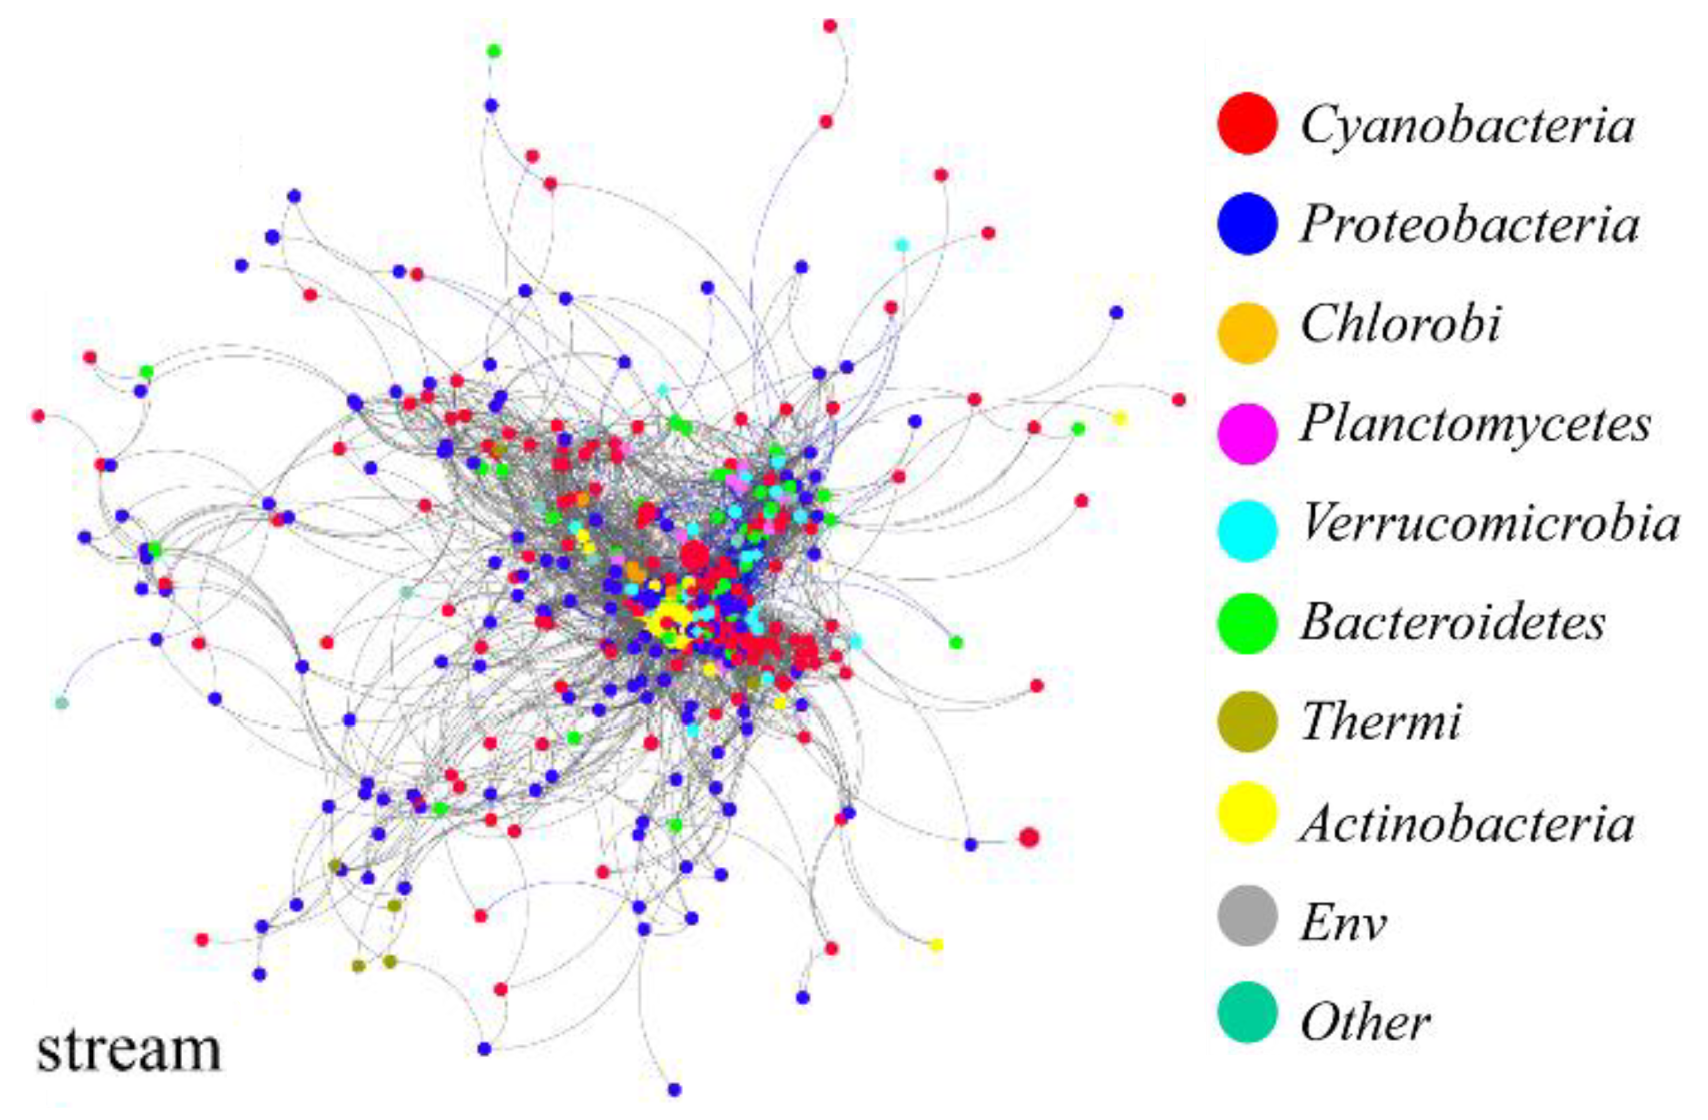
\includegraphics[width=\textwidth]{plots/cooccurrence_network}
 \end{center} 
  \end{block}
 \end{column}

 \begin{column}{0.5 \textwidth}
 \begin{block}{Bipartite network}
 \begin{center}
 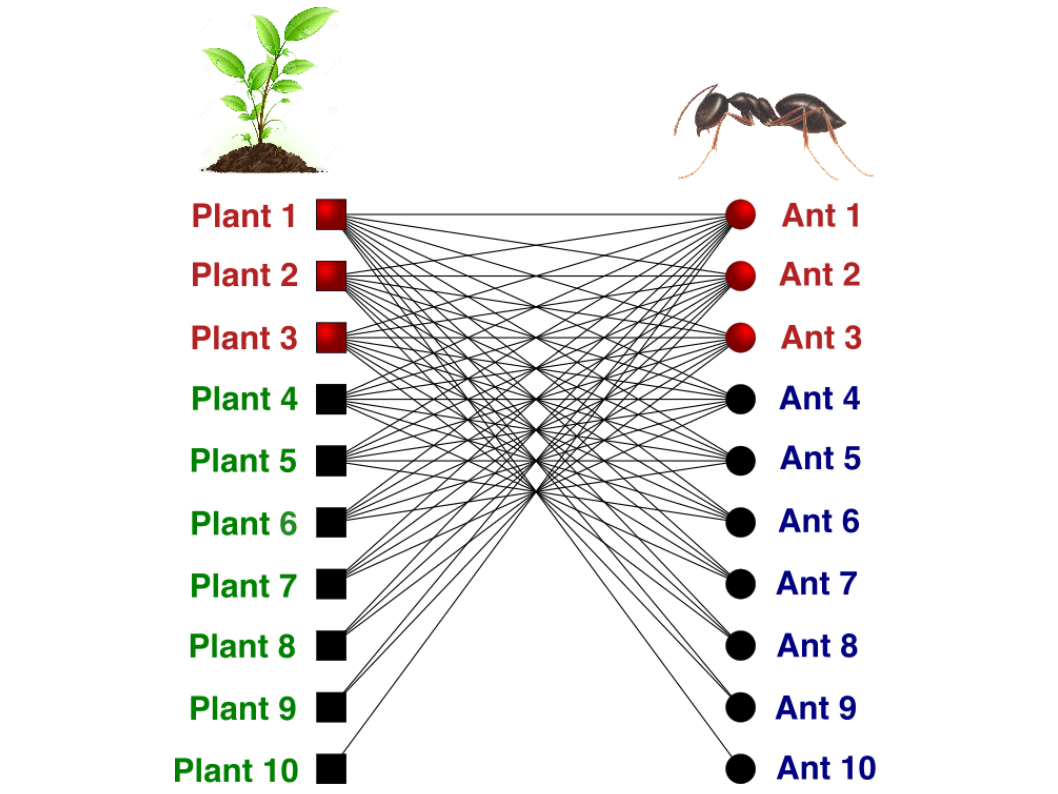
\includegraphics[width=\textwidth]{plots/plantant}
\end{center} 
 \end{block}
  \end{column}
\end{columns}


\end{frame}
 %==========================================
\begin{frame} \frametitle{Terminology}
 %==========================================
 
 A network consists in:
 \begin{itemize}
  \item nodes/vertices which represent individuals / species /ships which may interact or not,
  \item links/edges/connections which stand for an interaction between a pair of nodes / dyads.
  
 \end{itemize}

\bigskip
 
 A network may be 
 \begin{itemize}
  \item directed / oriented (e.g. food web...),
  \item symmetric / undirected (e.g. coexistence network),
  \item with or without loops.
 \end{itemize}

This distinction only makes sense for simple networks (not bipartite).
 
 
\end{frame}


 %==========================================
\begin{frame}\frametitle{Network representation and adjacency matrix}
 %==========================================
For a non-directed network
 \begin{columns}
 \begin{column}{.45\paperwidth}
$$Y=\left(
\begin{array}{rrrrr}
 0 & 1 & 0 & 1 \\ 
 1 & 0 & 1 & 1 \\ 
 0 & 1 & 0 & 0 \\ 
 1 & 1 & 0 & 0 \\ 
\end{array}\right)
$$
\end{column}

\begin{column}{.5\paperwidth}

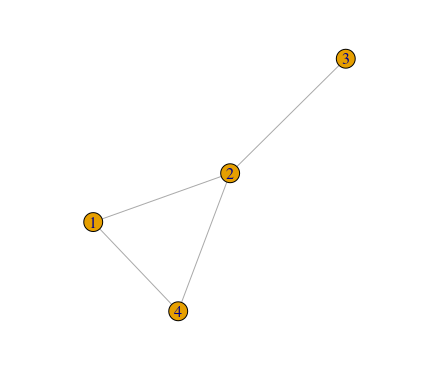
\includegraphics[scale=.5]{graphe_adj.png}

\end{column}

\end{columns}

\begin{itemize}
\item $n$ rows and $n$ columns,
\item symmetric   matrix
\end{itemize}

\end{frame}
%==========================================
\begin{frame}\frametitle{Network representation and adjacency matrix}
%==========================================
 
For a directed network
 \begin{columns}
 \begin{column}{.45\paperwidth}
$$Y=\left(
\begin{array}{rrrrr}
0 & 1 & 1 & 1 \\ 
 1 & 0 & 0 & 1 \\ 
 1 & 0 & 0 & 0 \\ 
 0 & 0 & 0 & 0 \\ 
\end{array}\right)
$$
\end{column}

\begin{column}{.5\paperwidth}

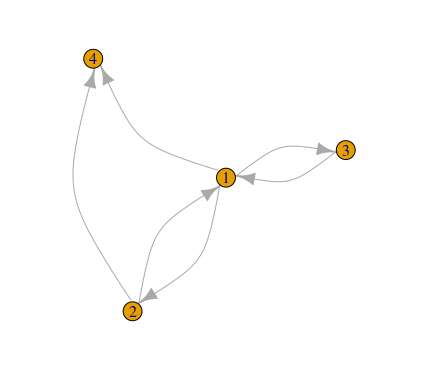
\includegraphics[scale=.5]{graphe_adj_dir.png}

\end{column}

\end{columns}

\begin{itemize}
\item $n$ rows and $n$ columns,
\item non symmetric   matrix
\end{itemize}

\end{frame}
%======================================================
\begin{frame}\frametitle{Bipartite network and incidence matrix}
%=====================================================
 \begin{columns}
 \begin{column}{.45\paperwidth}
$$Y=\left(
\begin{array}{rrrrrrr}
0 &   0 &   1 &   1 &   0 &   0 &   0 \\ 
   0 &   1 &   0 &   0 &   1 &   1 &   0 \\ 
   0 &   0 &   1 &   0 &   0 &   0 &   0 \\ 
  0 &   0 &   0 &   0 &   1 &   1 &   0 \\ 
\end{array}\right)
$$


\begin{itemize}
 \item n rows and m columns, rectangular matrix.
 \end{itemize}
\end{column}
\begin{column}{.5\paperwidth}

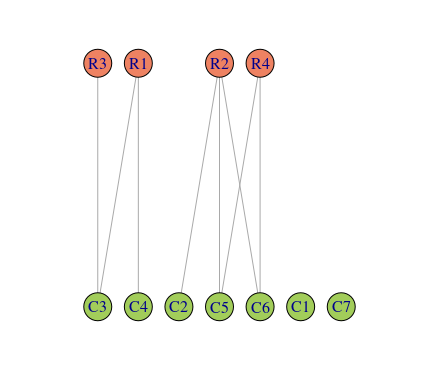
\includegraphics[scale=.5]{graphe_bipartite.png}

\end{column}

\end{columns}
\end{frame}
%======================================================
\begin{frame}\frametitle{Available data}
%======================================================
 
\begin{center}
 \includegraphics[scale=1]{plots/image_SBM.png}
\end{center}

\begin{itemize}
 \item  the network provided as:
\begin{itemize}
 \item an adjacency matrix (for simple network) or an incidence matrix (for bipartite network),
 \item a list of pair of nodes / dyads which are linked.
\end{itemize}

\item some additional covariates on nodes, dyads which can account for sampling effort.
 \end{itemize}






\end{frame}

%======================================================
\begin{frame}\frametitle{Goal}
%======================================================

 
\begin{center}
 \includegraphics[scale=.6]{image_SBM.png}
\end{center}

\begin{itemize}
 \item Unraveling / describing / modeling the network topology. 
 \item Discovering particular structure of interaction between some subsets of nodes.
 \item Understanding network heterogeneity.
 \item Not inferring the network !
 \end{itemize}


\end{frame}
%======================================================
\section{Descriptive statistics}
%======================================================


%====================================================================
   \begin{frame}{Network analysis}
 %====================================================================
\myemph{Aim} : give a short description of the network, give a hint about its structure, look  for heterogeneity in the connections
\begin{itemize}
\item Many metrics supplied for simple networks
\item Have been extended to bipartite networks
\end{itemize}
\end{frame}


%====================================================================
\begin{frame}{Example : Chilean foodweb}
 %====================================================================

\cite{kefi}

\centering
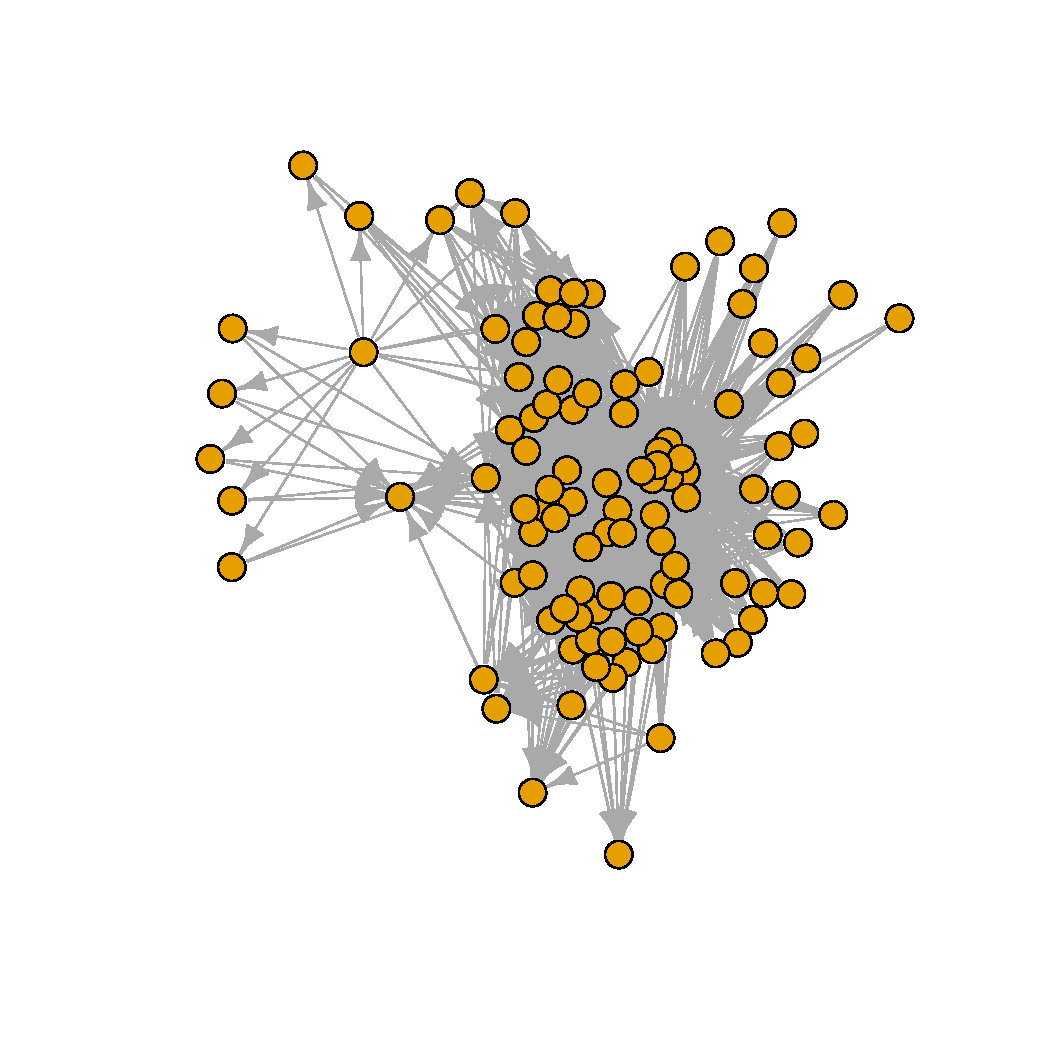
\includegraphics[width=0.7\textwidth]{plots/chilean_food_web}

\begin{itemize}
 \item $n=106$ species / nodes,
 \item density of edges: $12.1\%$.
\end{itemize}


\end{frame}


%====================================================================
\begin{frame}{Degree} 
%====================================================================
$$
\begin{array}{cclccl}
\mbox{deg}(u) &=& \sum_{v \in V} (u \leftrightarrow v), \quad &\mbox{deg}(v) &=& \sum_{u \in U} (u \leftrightarrow v)\\
\mbox{deg}_i &=& \sum_{ j  = 1}^{|V|} Y_{ij}&\mbox{deg}_j&=& \sum_{ i  = 1}^{|U|} Y_{ij}
\end{array}
$$

\begin{itemize}
\item Nodes with high degree are \alert{hubs}
\item Nodes with null degree are \alert{isolated}
\item If edges are oriented : in- and out- degrees can be computed. 
\end{itemize}
\end{frame}
%====================================================================
\begin{frame}{Degrees on Chilean foodweb} 
%====================================================================


\centering
\begin{columns}
\begin{column}{0.5\textwidth}
 \begin{block}{Out degree distribution}
  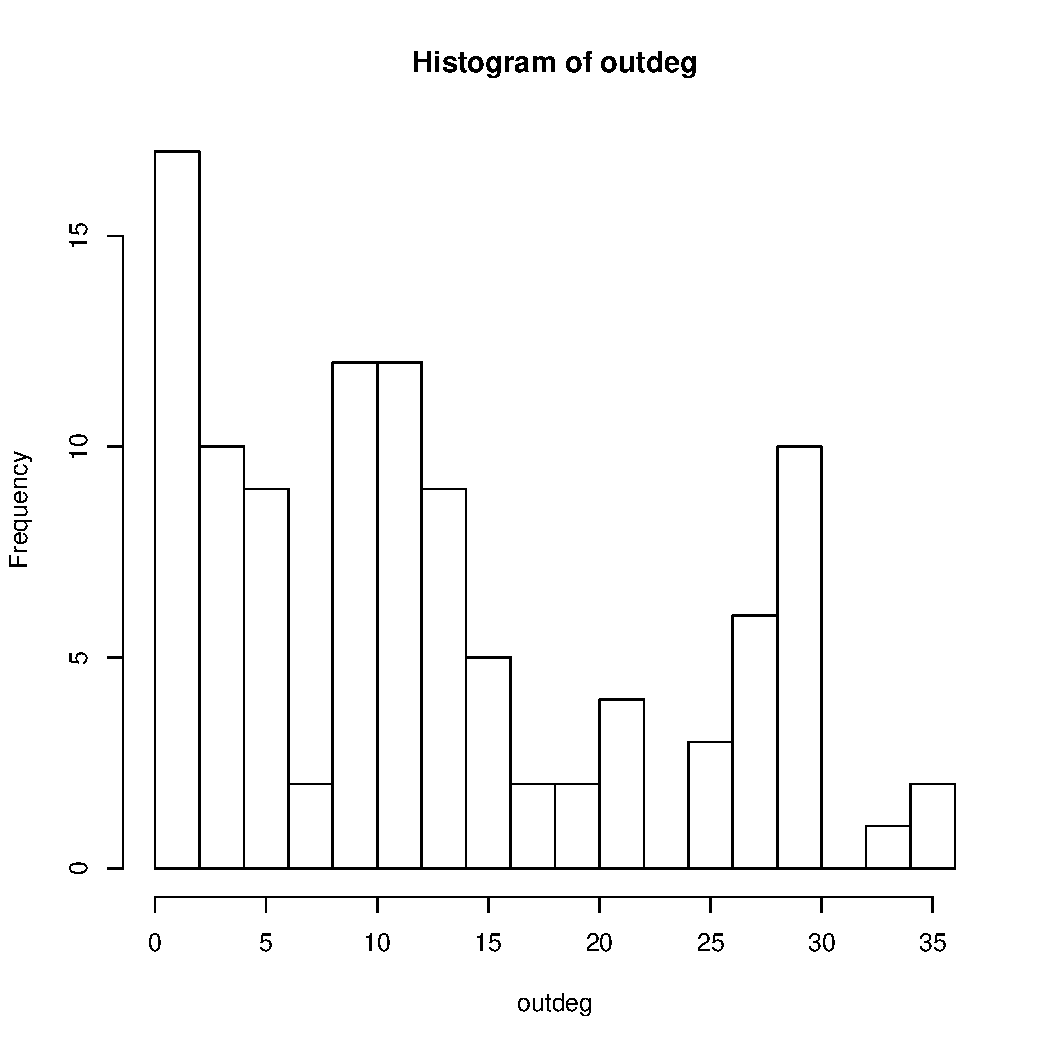
\includegraphics[width= \textwidth]{chilean_outdeg}
 \end{block}
\end{column}
 \begin{column}{0.5\textwidth}
 \begin{block}{In degree distribution}
  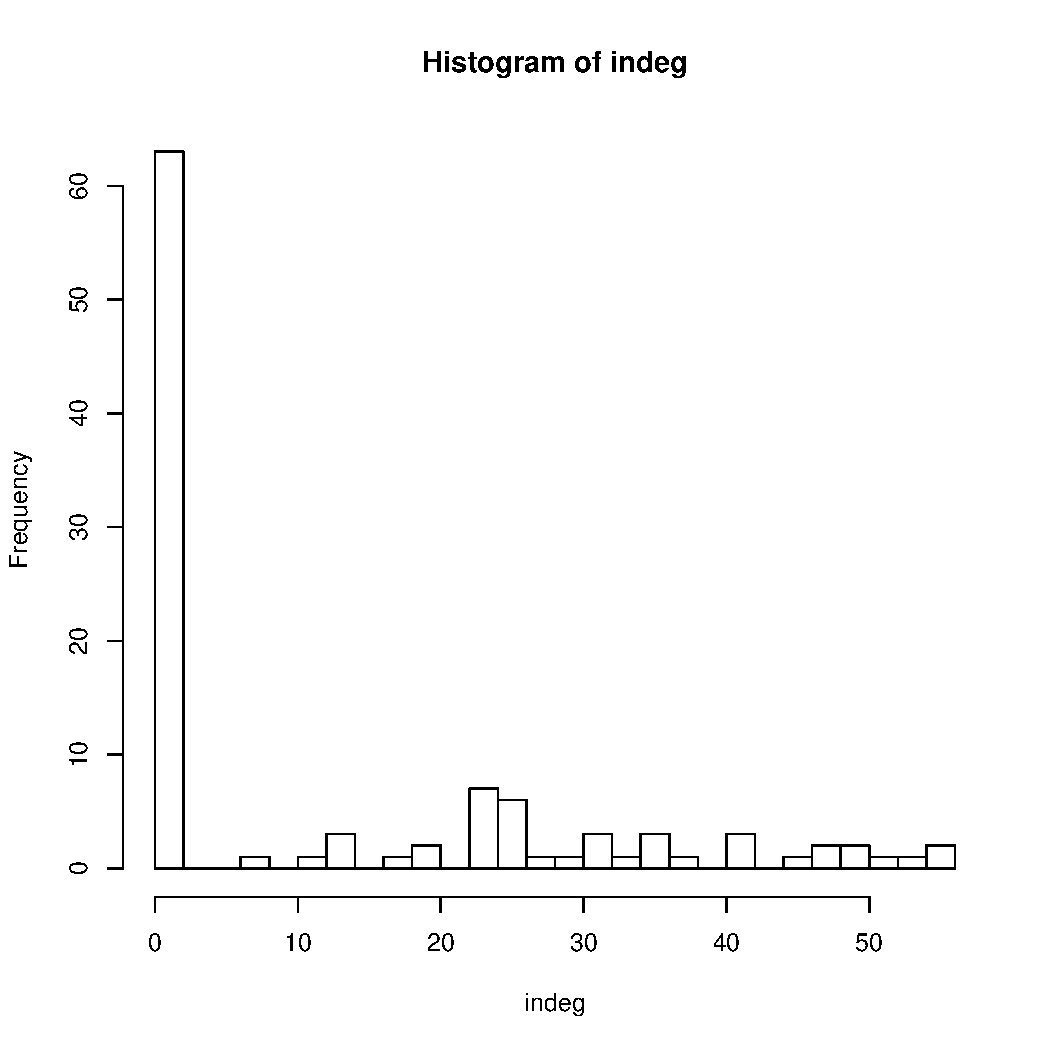
\includegraphics[width= \textwidth]{chilean_intdeg}
 \end{block}
\end{column}

 
\end{columns}

\end{frame}

%====================================================================
\frame{\frametitle{Closeness centrality} 
%====================================================================

Property on a node

\begin{block}{Definition}
Determine whether a node can communicate with other nodes of the network directly or through the short paths.

$$C(u) = \frac{1}{\sum_{w \in U  \cup V} d(u,w)}$$ 

where $d(u,w)$ is the length of the shortest path between $u$ and $w$ (through the network). 
\end{block}

Note that, for bipartite networks
\begin{itemize}
\item A node  $ u \in U$ can have a minimum distance of $1$ with $v \in V$. 
\item A node  $ u \in U$ can have a minimum distance of $2$ with $u' \in U$.
\item All paths between nodes of the same set are of even length.
\end{itemize}

}


%====================================================================
\frame{\frametitle{Betweenness centrality} 
%====================================================================
Property on a node
\begin{block}{Definition}
Betweenness centrality quantifies the number of times a node acts as a bridge along the shortest path between two other nodes.
\end{block}

The betweenness of a vertex $ v$ is computed as follows. 
\begin{itemize}
\item  For each pair of vertices $(w,w')$, compute the shortest paths between them. $\delta_{w,w'}$ is the number of shortest paths between $(w,w')$
\item  For each pair of vertices $(w,w')$, determine the fraction of shortest paths that pass through $v$ : $\frac{\delta_{w,w'}(v)}{\delta_{w,w'}}$
\item  Sum this fraction over all pairs of vertices $(w,w')$.
$$ B(v) = \sum_{w  \neq w' \neq v} \frac{\delta_{w,w'}(v)}{\delta_{w,w'}}$$
\end{itemize}
}


%====================================================================
\frame{\frametitle{Betweenness centrality} 
%====================================================================
\centering
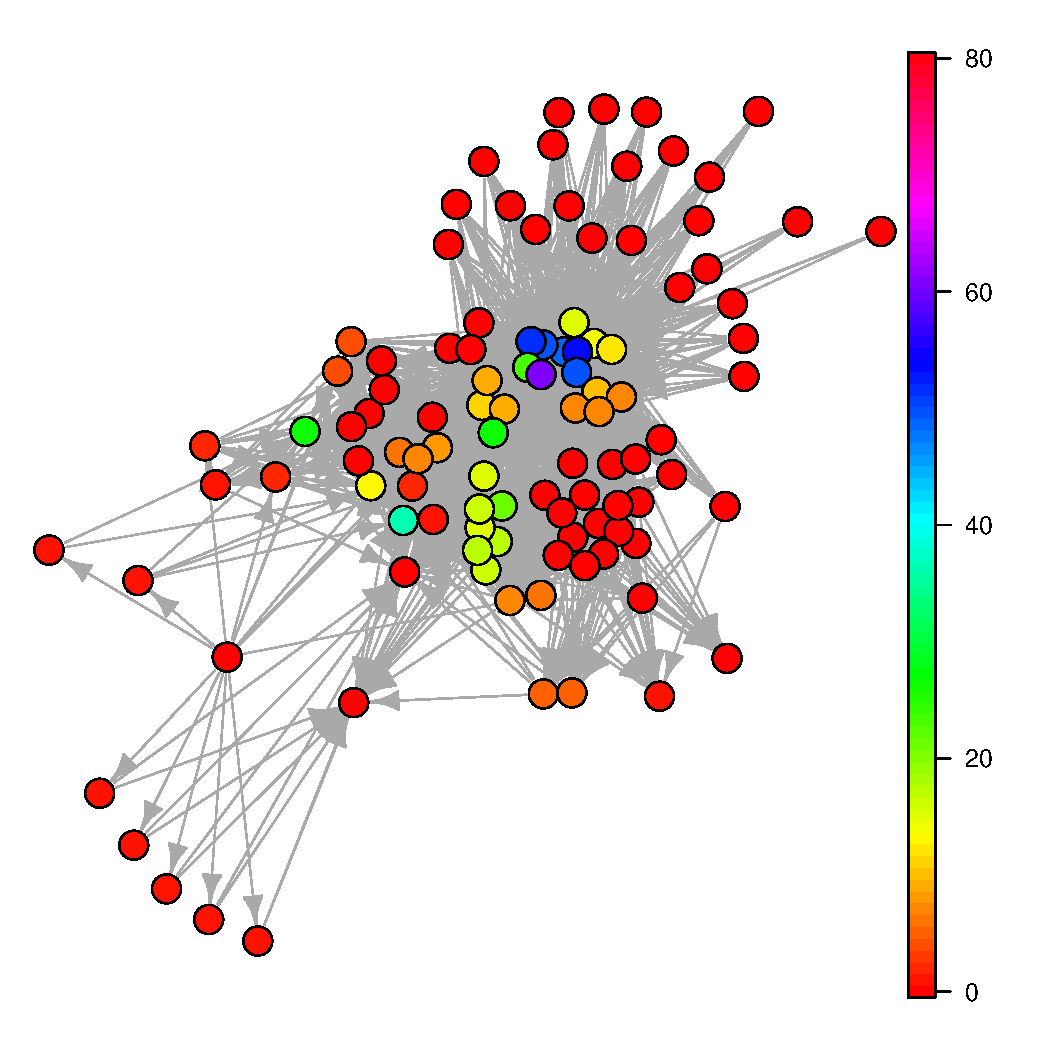
\includegraphics[width=0.6\textwidth]{chilean_between}

\begin{tabular}{cccccc}
   Min. & 1st Qu. & Median  &  Mean & 3rd Qu. &    Max.\\ 
 0.000 &  0.000&   0.000 &  6.604 &  6.929&  59.570
\end{tabular} 

}

%====================================================================


%====================================================================
\frame{\frametitle{Nestedness} 
%====================================================================

Property on the network
\begin{block}{Definition}
\begin{itemize}
\item Important property in ecology
\item Defined as a pattern of interactions in which specialists (e.g. pollinators that visit few plant species) interact with plants that are visited by generalists.  
\item Mathematically, looking for a reordering of rows and columns such that $Y$ is nested
\end{itemize}

\end{block}
}

%====================================================================
\frame{\frametitle{Nestedness} 
%====================================================================
\begin{center}
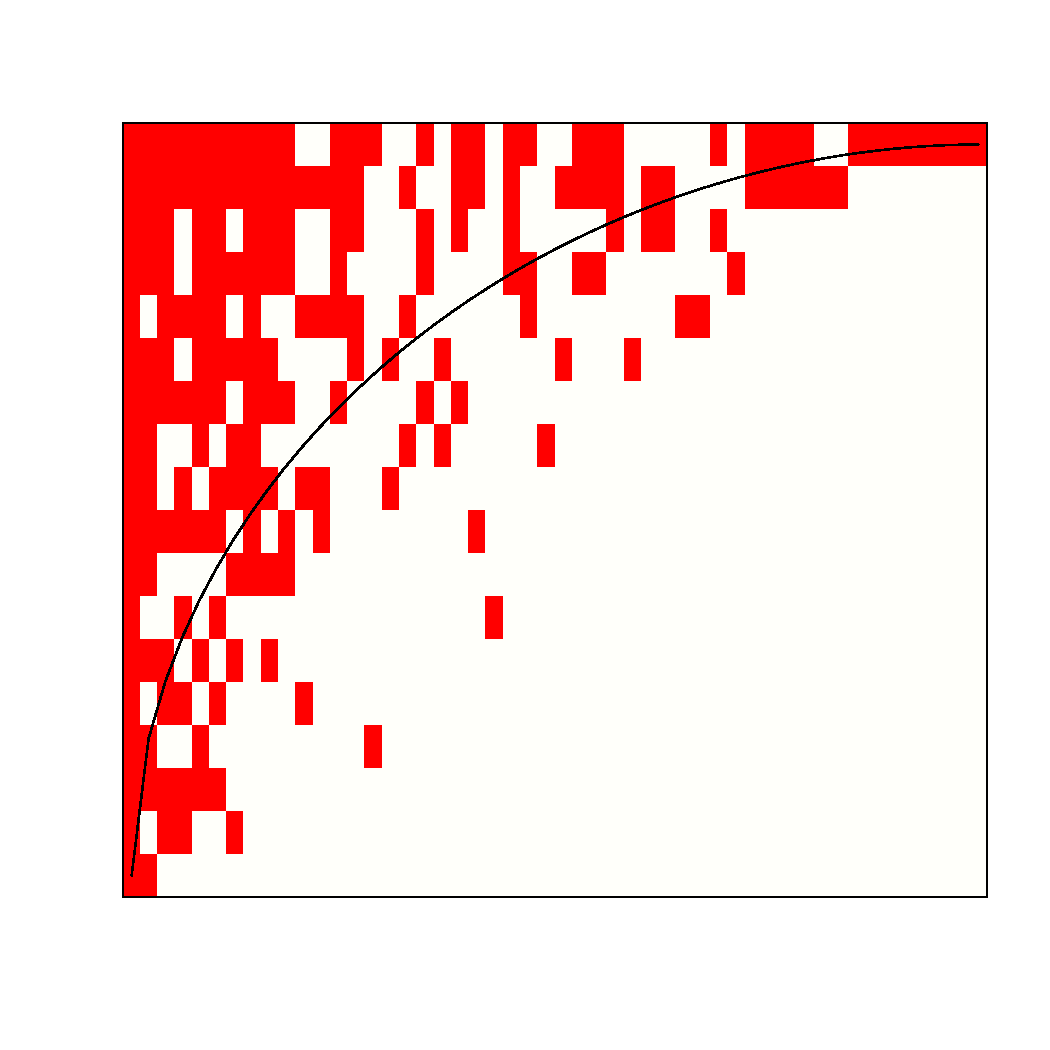
\includegraphics[width = 0.5 \textwidth]{chilean_nested}
\end{center}
 \begin{itemize}
  \item more generally used on incidence matrices,
  \item significance of the nestedness index computed by random permutations of the matrix,
  \item this food web is found to be nested.
\end{itemize}
}

%====================================================================
\frame{\frametitle{Modularity} 
%====================================================================
Property on the network
\begin{block}{Definition}
Existence of clusters (blocks, module, communities) where nodes are much more connected than with other clusters
\end{block}
}



%====================================================================
\frame{\frametitle{Modularity} 
%====================================================================
\centering
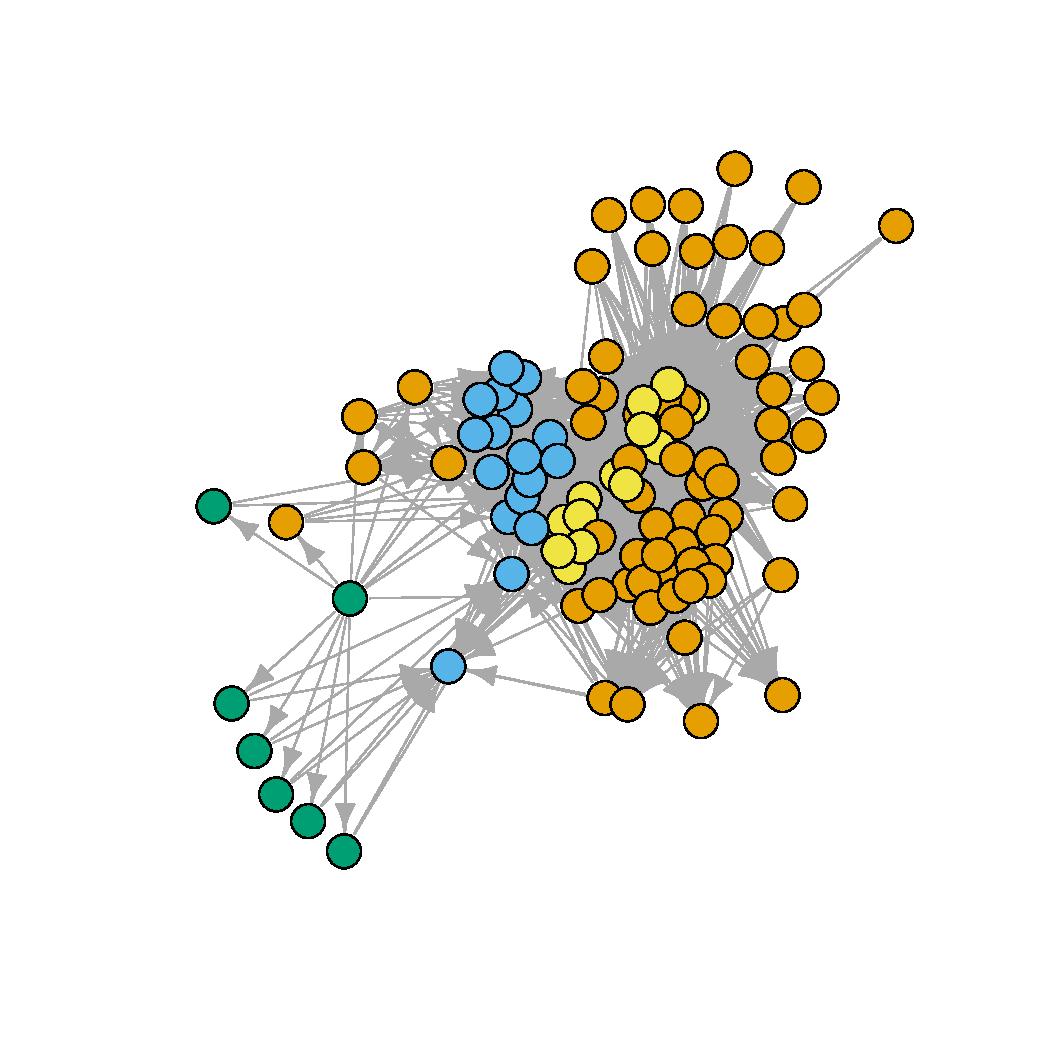
\includegraphics[width=0.6\textwidth]{chilean_modularity}

 \begin{itemize}
  \item
  \begin{tabular}{rrrrr}
  \hline
 1 & 2 & 3 & 4 \\ 
  \hline
  69 &  17 &   7 &  13 \\ 
   \hline
\end{tabular}
\item very low modularity.
 \end{itemize}

}




%====================================================================
\section{Probabilistic  model}
%====================================================================
\begin{frame}{Probabilistic approach}
\begin{itemize}
\item 
\alert{Context}: our   matrix $Y$ is the realization of a stochastic process.
\item 
\alert{Aim}: Propose a  stochastic process is able to mimic heterogeneity in the connections.  
\item \alert{Advantage}: benefit from the statistical tools (tests,  model selection, etc...)  
\end{itemize}

\end{frame}



%====================================================================
\begin{frame}\frametitle{A first random graph model for network: null model}
%====================================================================


\cite{erdos59a} Model for $n$ nodes 

$$\forall 1\le i,j\le n,\quad Y_{ij}\overset{i.i.d.}{\sim} b(p),$$
where $b$ is the Bernoulli distribution and $p\in[0,1]$ a probability for a link to exist. 


\begin{center}
 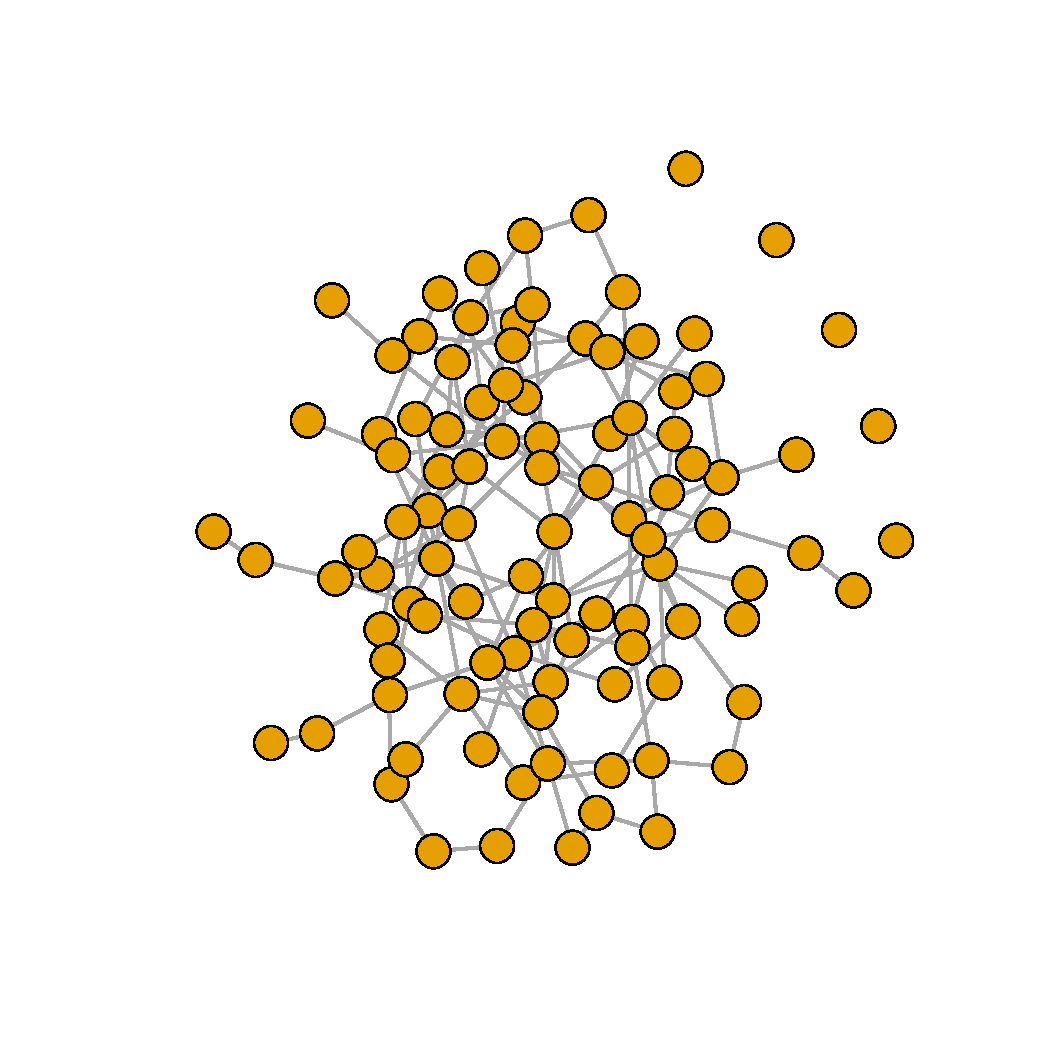
\includegraphics[scale=.3]{ER.pdf} 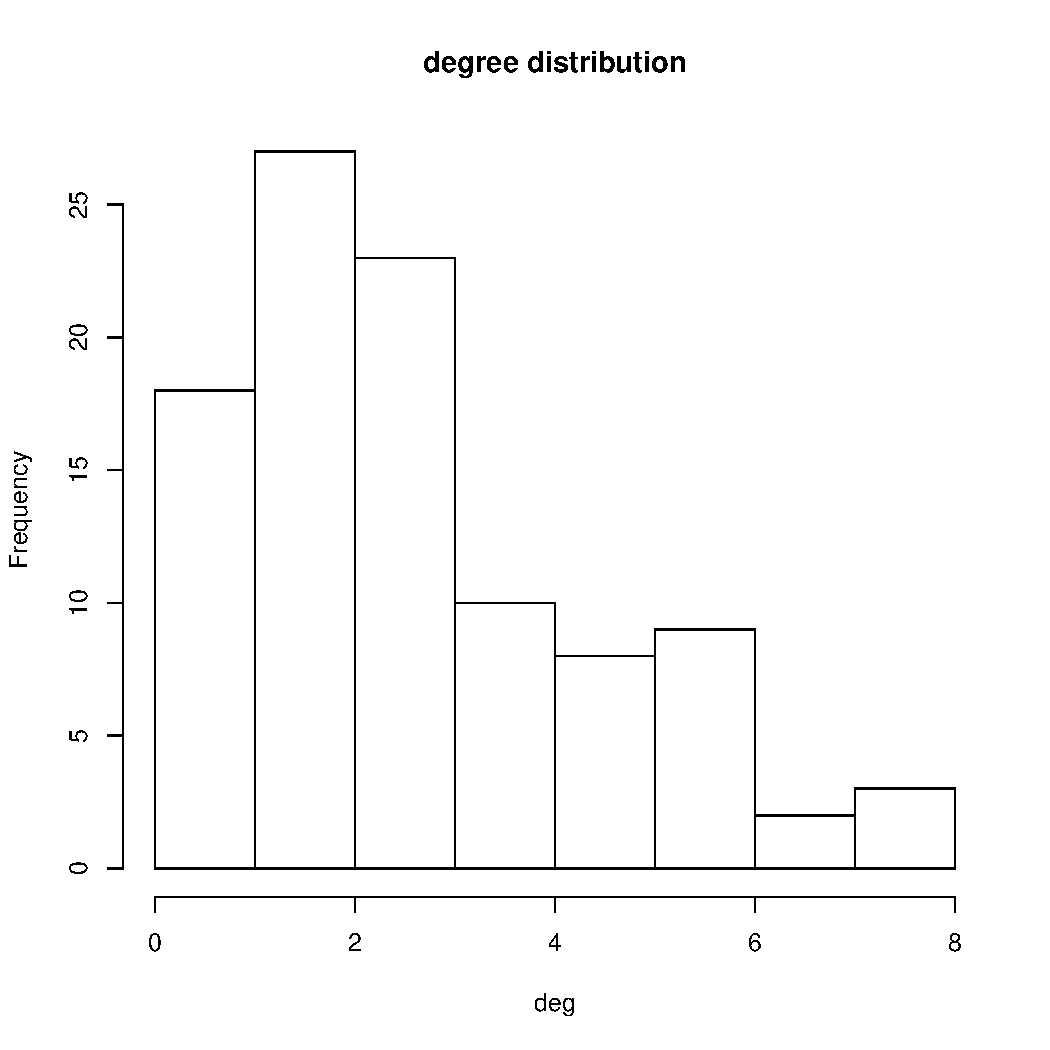
\includegraphics[scale=.3]{degER.pdf}
\end{center}


\end{frame}



%====================================================================
\begin{frame} \frametitle{Limitations of an ER graph to describe real networks}
%==================================================================== 
 
 
\begin{itemize}
\item  Homogeneity of the connections
 \item Degree distribution too concentrated, no high degree nodes,
 \item All nodes are equivalent (no nestedness...),
 \item No modularity, no hubs
 \end{itemize}

\end{frame}



%====================================================================
\subsection[SBM]{Stochastic Block Model}
%====================================================================


%====================================================================
\begin{frame}  \frametitle{Stochastic Block Model}
%====================================================================
 \cite{nowickiSnijders2001} 
Let ($Y_{ij}$) be an adjacency matrix 

\begin{block}{Latent variables}
\begin{itemize}
\item The nodes $i= 1,\dots,n$ are partitionned into $K$ clusters
\item $Z_i = k$ if node $i$ belongs to cluster (block) $k$
\item $Z_i$ independant variables
$$ \mathbb{P}(Z_i = k) = \pi_k$$
\end{itemize}
\end{block}

\begin{block}{Conditionally to $(Z_i)_{i=1,\dots,n}$... }

$(Y_{ij})$ independant and 
\begin{eqnarray*}
 Y_{ij}  | Z_i, Z_j \sim  \mathcal{B}ern(\alpha_{Z_i,Z_j}) \quad \Leftrightarrow \quad  P(Y_{ij} = 1 | Z_i = k, Z_j = \ell)  =  \alpha_{k\ell}
\end{eqnarray*}
\end{block}
 


\end{frame}



%====================================================================
\begin{frame} \frametitle{Stochastic Block Model : illustration}
%====================================================================
  \begin{center}
    \begin{overlayarea}{\textwidth}{.5\textheight}
      \begin{columns}
        \begin{column}{.45\paperwidth}
        \begin{tikzpicture}
          %% UN GRAPH

          \tikzstyle{every edge}=[-,>=stealth',shorten >=1pt,auto,thin,draw]
          \tikzstyle{every state}=[draw=none,text=white,scale=0.65, font=\scriptsize, transform shape]
          \tikzstyle{every node}=[fill=yellow!40!orange]
          % premier cluster
          \node[state] (A1) at (0,0.5) {A1};
          \node[state] (A2) at (1,0.5) {A2};
          \node[state] (A3) at (.5,1.5) {A3};

          \path (A2) edge [bend left] node[fill=white,below=.1cm]
          {$\alpha_{\textcolor{yellow!40!orange}{\bullet}\textcolor{yellow!40!orange}{\bullet}}$}
          (A1)
          (A1) edge [bend left] (A3)
          (A3) edge [bend left] (A2);

          \tikzstyle{every node}=[fill=blue!80!black]
          \foreach \angle/\text in {234/B1, 162/B2, 90/B3, 18/B4, -54/B5} {
            \node[fill=blue,state,xshift=5cm,yshift=3.5cm]     (\text)    at
            (\angle:1cm) {\text};
          }
          \path (B2) edge (B5)
          (B1) edge (B4);
          \foreach \from/\to in {1/2,2/3,4/5,5/1}{
            \path (B\from) edge [bend left] (B\to);
          }

          \path    (B3)    edge     [bend    left]    node[fill=white]
          {$\alpha_{\textcolor{blue!80!black}{\bullet}\textcolor{blue!80!black}{\bullet}}$}  (B4) ;
          
          \tikzstyle{every node}=[fill=green!50!black]
          % troisieme cluster
          \node[state] (C1) at (3,-.5) {C1};
          \node[state] (C2) at (4,0) {C2};

          \path (C1) edge [bend right] node[fill=white,below=.25cm]
          {$\alpha_{\textcolor{green!50!black}{\bullet}\textcolor{green!50!black}{\bullet}}$}
          (C2);

          % inter cluster
          \path (A3) edge [bend right]  (B2)
          (A3)    edge    [bend    left]    node[fill=white]
          {$\alpha_{\textcolor{yellow!40!orange}{\bullet}\textcolor{blue!80!black}{\bullet}}$}
          (B3)
          (C2) edge [bend right] node[fill=white,right]
          {$\alpha_{\textcolor{blue!80!black}{\bullet}\textcolor{green!50!black}{\bullet}}$}
          (B4)
          (A2) edge [bend right] node[fill=white]
          {$\alpha_{\textcolor{yellow!40!orange}{\bullet}\textcolor{green!50!black}{\bullet}}$}
          (C1);
        \end{tikzpicture}
        \end{column}


        \begin{column}{.5\paperwidth}
          \begin{small}
            \begin{block}{Parameters}
              Let $n$ nodes divided into $3$ clusters
              \begin{itemize}
              \item
                $\mathcal{K}=\{\textcolor{yellow!40!orange}{\bullet},\textcolor{blue!80!black}{\bullet},\textcolor{green!50!black}{\bullet}\}$
                 clusters
              \item  $\pi_\bullet  =  \mathbb{P}(i  \in  \bullet)$,
                $\bullet\in\mathcal{K},i=1,\dots,n$
              \item      $\alpha_{\textcolor{yellow!40!orange}{\bullet}\textcolor{blue!80!black}{\bullet}}     =      \mathbb{P}(i
                \leftrightarrow j | i\in\textcolor{yellow!40!orange}{\bullet},j\in\textcolor{blue!80!black}{\bullet})$
              \end{itemize}
            \end{block}
          \end{small}
        \end{column}
      \end{columns}
    \end{overlayarea}
  \end{center}
  
%\begin{eqnarray*}
%&(Z_i) &  \ \sim^{\text{iid}} \mathcal{M}(1,\alpha) \ \text{et} \  Z_{i} \in \{1,...,Q\}, \\ 
% &(Y_{ij})&| \ \{Z_{i},Z_{j}\} \sim^{\text{ind}} \mathcal{B}(\pi_{Z_{i}Z_{j}}).\\
%\end{eqnarray*}

% Proposition Julien
\begin{align*}
Z_i = \mathbf{1}_{\{i \in \bullet\}}  \ & \sim^{\text{iid}} \mathcal{M}(1,\pi), \quad \forall\bullet \in \mathcal{K}, \\ 
Y_{ij} \ | \ \{i\in\textcolor{yellow!40!orange}{\bullet},j\in\textcolor{blue!80!black}{\bullet}\}
& \sim^{\text{ind}} \mathcal{B}(\alpha_{\textcolor{yellow!40!orange}{\bullet}\textcolor{blue!80!black}{\bullet}})\\
\end{align*}

\end{frame}


%====================================================================
\begin{frame}{DAG of the model}
%====================================================================

 \begin{center}
%   \includegraphics[scale=.3, clip=true, trim=0 335 65 0]{../Figures/HMModel}
  \begin{tikzpicture}
  \node[hidden] (Z1) at (0*\edgeunit, 2*\edgeunit) {$Z_1$};
  \node[hidden] (Z2) at (-2*\edgeunit,  0.5*\edgeunit) {$Z_2$};
 \node[hidden] (Z3) at (2*\edgeunit, 0*\edgeunit) {$Z_3$};

 
  \node[observed] (Y12) at (0*\edgeunit, 1*\edgeunit) {$Y_{12}$};
 \node[observed] (Y13) at (1*\edgeunit, 1*\edgeunit) {$Y_{13}$};
  \node[observed] (Y21) at (-1*\edgeunit, 0*\edgeunit) {$Y_{21}$};

  \node[observed] (Y23) at (1*\edgeunit, 0*\edgeunit) {$Y_{23}$};

  \node[observed] (Y31) at (-1*\edgeunit, -1*\edgeunit) {$Y_{31}$}; 
  \node[observed] (Y32) at (0*\edgeunit, -1*\edgeunit) {$Y_{32}$};


 
  \draw[arrow] (Z1) to (Y12);
  \draw[arrow] (Z1) to (Y21);
  \draw[arrow] (Z1) to (Y31);
  \draw[arrow] (Z1) to (Y13);
  
  \draw[arrow] (Z2) to (Y23);
  \draw[arrow] (Z2) to (Y32);
 
  \draw[arrow] (Z2) to (Y12);
  \draw[arrow] (Z2) to (Y21);
  
  
  \draw[arrow] (Z3) to (Y13);
  \draw[arrow] (Z3) to (Y23);
  \draw[arrow] (Z3) to (Y31);
  \draw[arrow] (Z3) to (Y32);
 
  
  \end{tikzpicture}
  \end{center}
  \end{frame}
%================================================================

%====================================================================
\begin{frame}\frametitle{SBM : A great generative model}
%====================================================================
\begin{itemize}
\item  Generative model : easy to simulate
\item No a priori on the type of structure
\item Combination of modularity, nestedness, etc... 
\end{itemize}
\end{frame}

%====================================================================
\begin{frame}\frametitle{Networks with hubs generated by SBM}
%====================================================================
\centering
 
 \begin{itemize}
  \item   $\pi = c(.15,.35,.15,.35)$
  \item $\alpha = \left(\begin{array}{cccc}
                          0.80 & 0.80 & 0.20 & 0.20 \\ 
   0.80 & 0.20 & 0.20 & 0.20 \\ 
    0.20 & 0.20 & 0.80 & 0.80 \\ 
    0.20 & 0.20 & 0.80 & 0.20  
                        \end{array}
 \right)$
 \end{itemize}
 
\centering
\begin{tabular}{cc}
 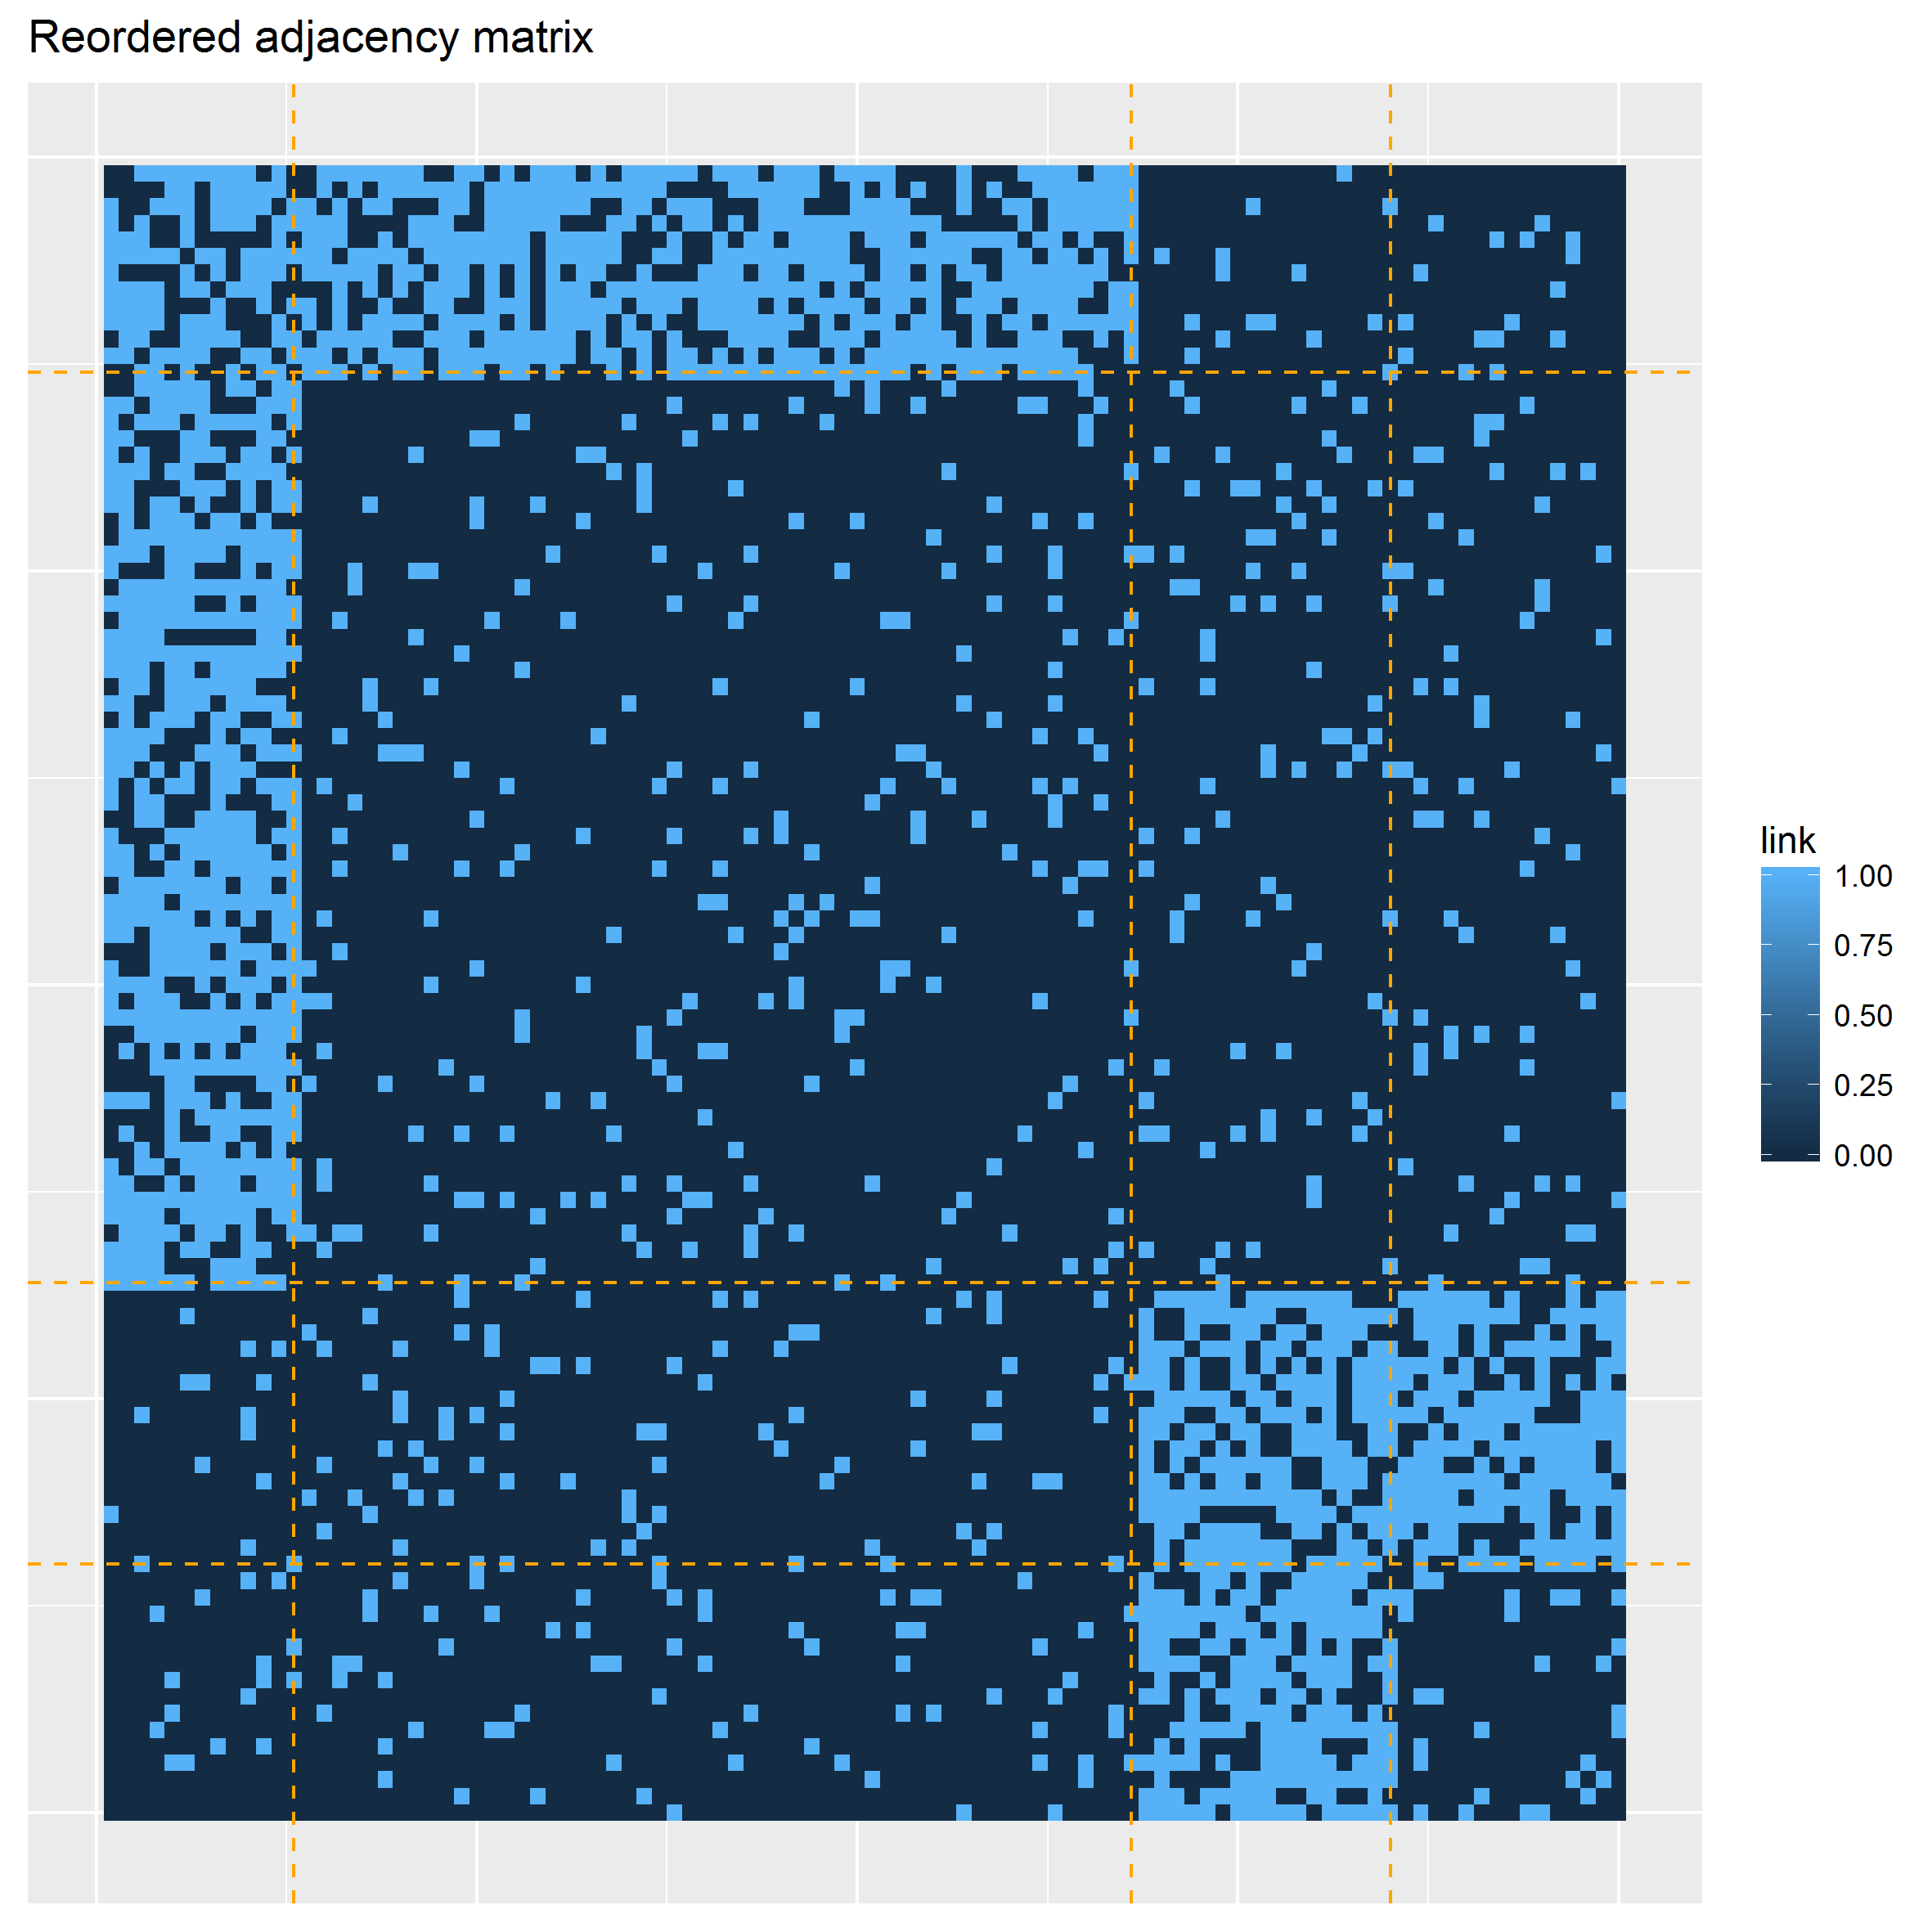
\includegraphics[scale=.2]{sbm/Etoile_reordered_adja_with_groups.png}&
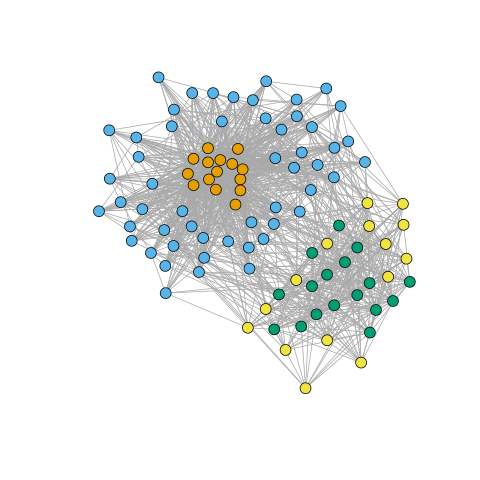
\includegraphics[scale=.2]{sbm/Etoile_graphe_with_colors.png}
  % 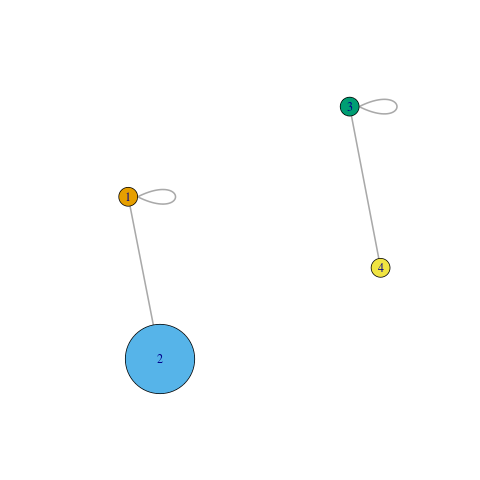
\includegraphics[scale=.2]{sbm/Etoile_graphe_resume.png}
 \end{tabular}

 

\end{frame}



%====================================================================
\begin{frame}\frametitle{Community network  generated by SBM}
%====================================================================
 \begin{itemize}
  \item   $\pi = c(0.25,0.35,0.40)$
  \item $\alpha = \left(\begin{array}{ccc}
                        0.80 & 0.20 & 0.20 \\ 
 0.20 & 0.80 & 0.20 \\ 
 0.20 & 0.20 & 0.80\end{array}
 \right)$
 \end{itemize}
 
\centering
\begin{tabular}{cc}
 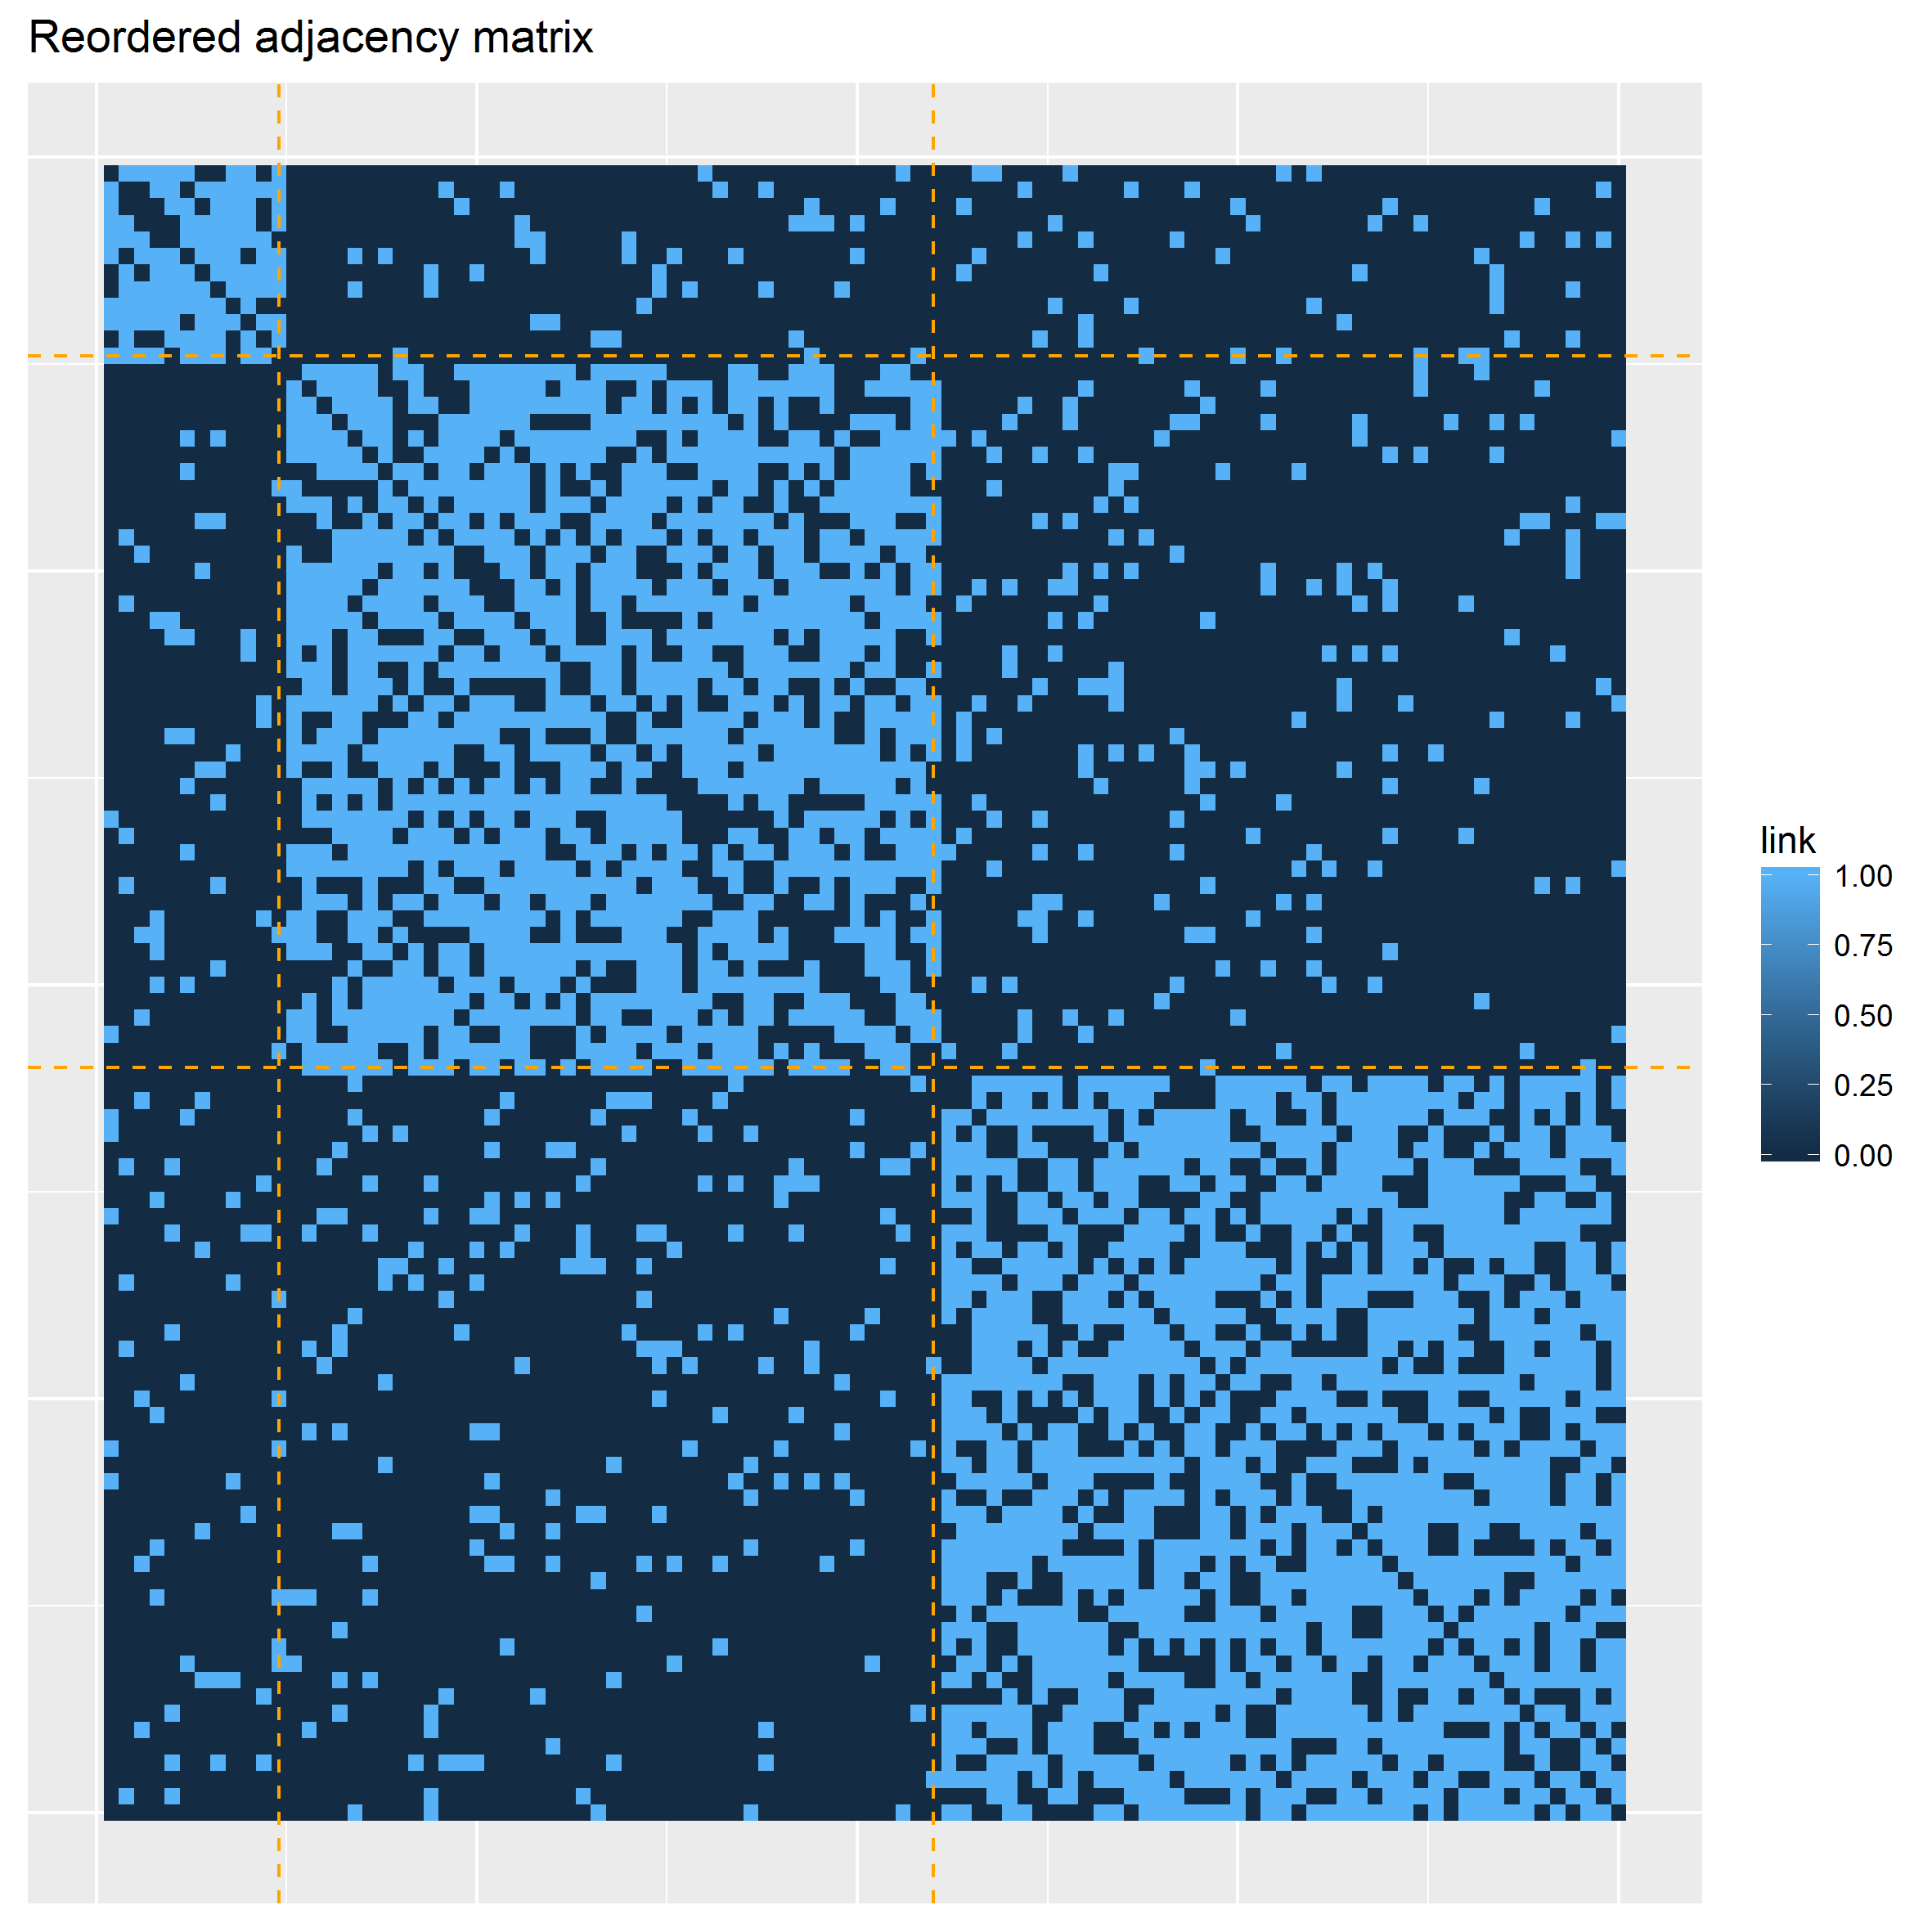
\includegraphics[scale=.2]{sbm/Affiliation_reordered_adja_with_groups.png}&
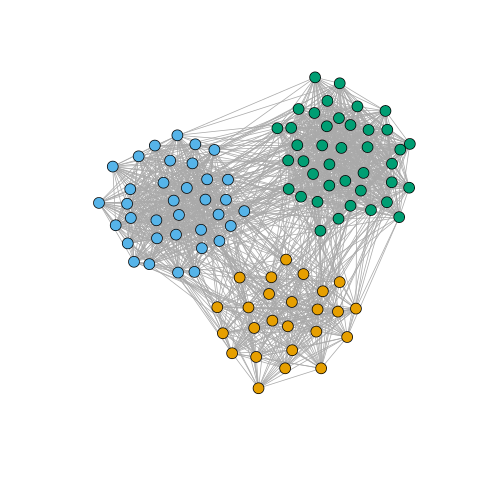
\includegraphics[scale=.2]{sbm/Affiliation_graphe_with_colors.png} 
 \end{tabular}
% 
% \begin{tabular}{cc}
%    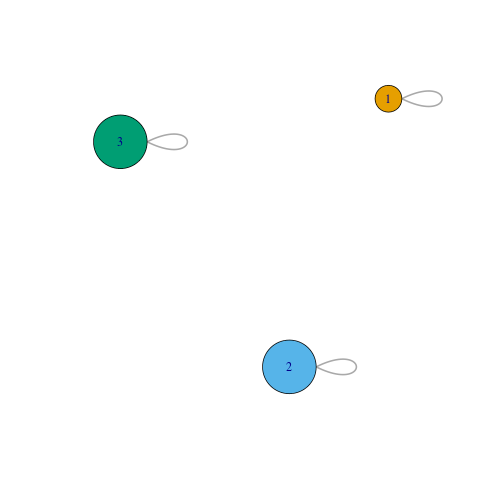
\includegraphics[scale=.2]{sbm/Affiliation_graphe_resume.png}
%     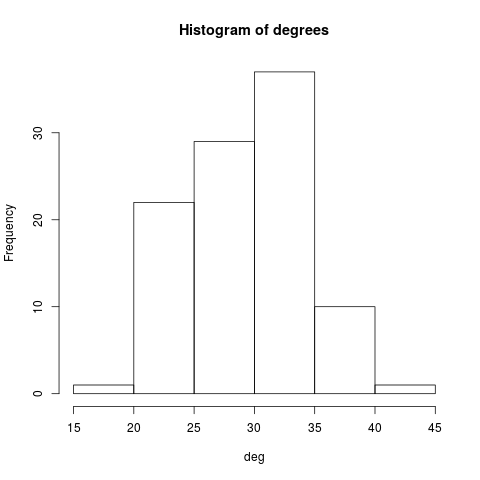
\includegraphics[scale=.2]{sbm/Affiliation_histogram_degree.png}&
%  \end{tabular}

\end{frame}


%====================================================================
\begin{frame}\frametitle{Nestedness  generated by SBM}
%====================================================================
\centering
 \begin{itemize}
  \item   $\pi = c(.15,.35,.15,.35)$
  \item $\alpha = \left(\begin{array}{cccc}
                          0.80 & 0.80 & 0.80 & 0.80 \\ 
    0.80 & 0.80 & 0.80 & 0.20 \\ 
    0.20 & 0.80 & 0.20 & 0.80 \\ 
    0.80 & 0.20 & 0.20 & 0.20  
                        \end{array}
 \right)$
 \end{itemize}
 
\centering
\begin{tabular}{cc}
 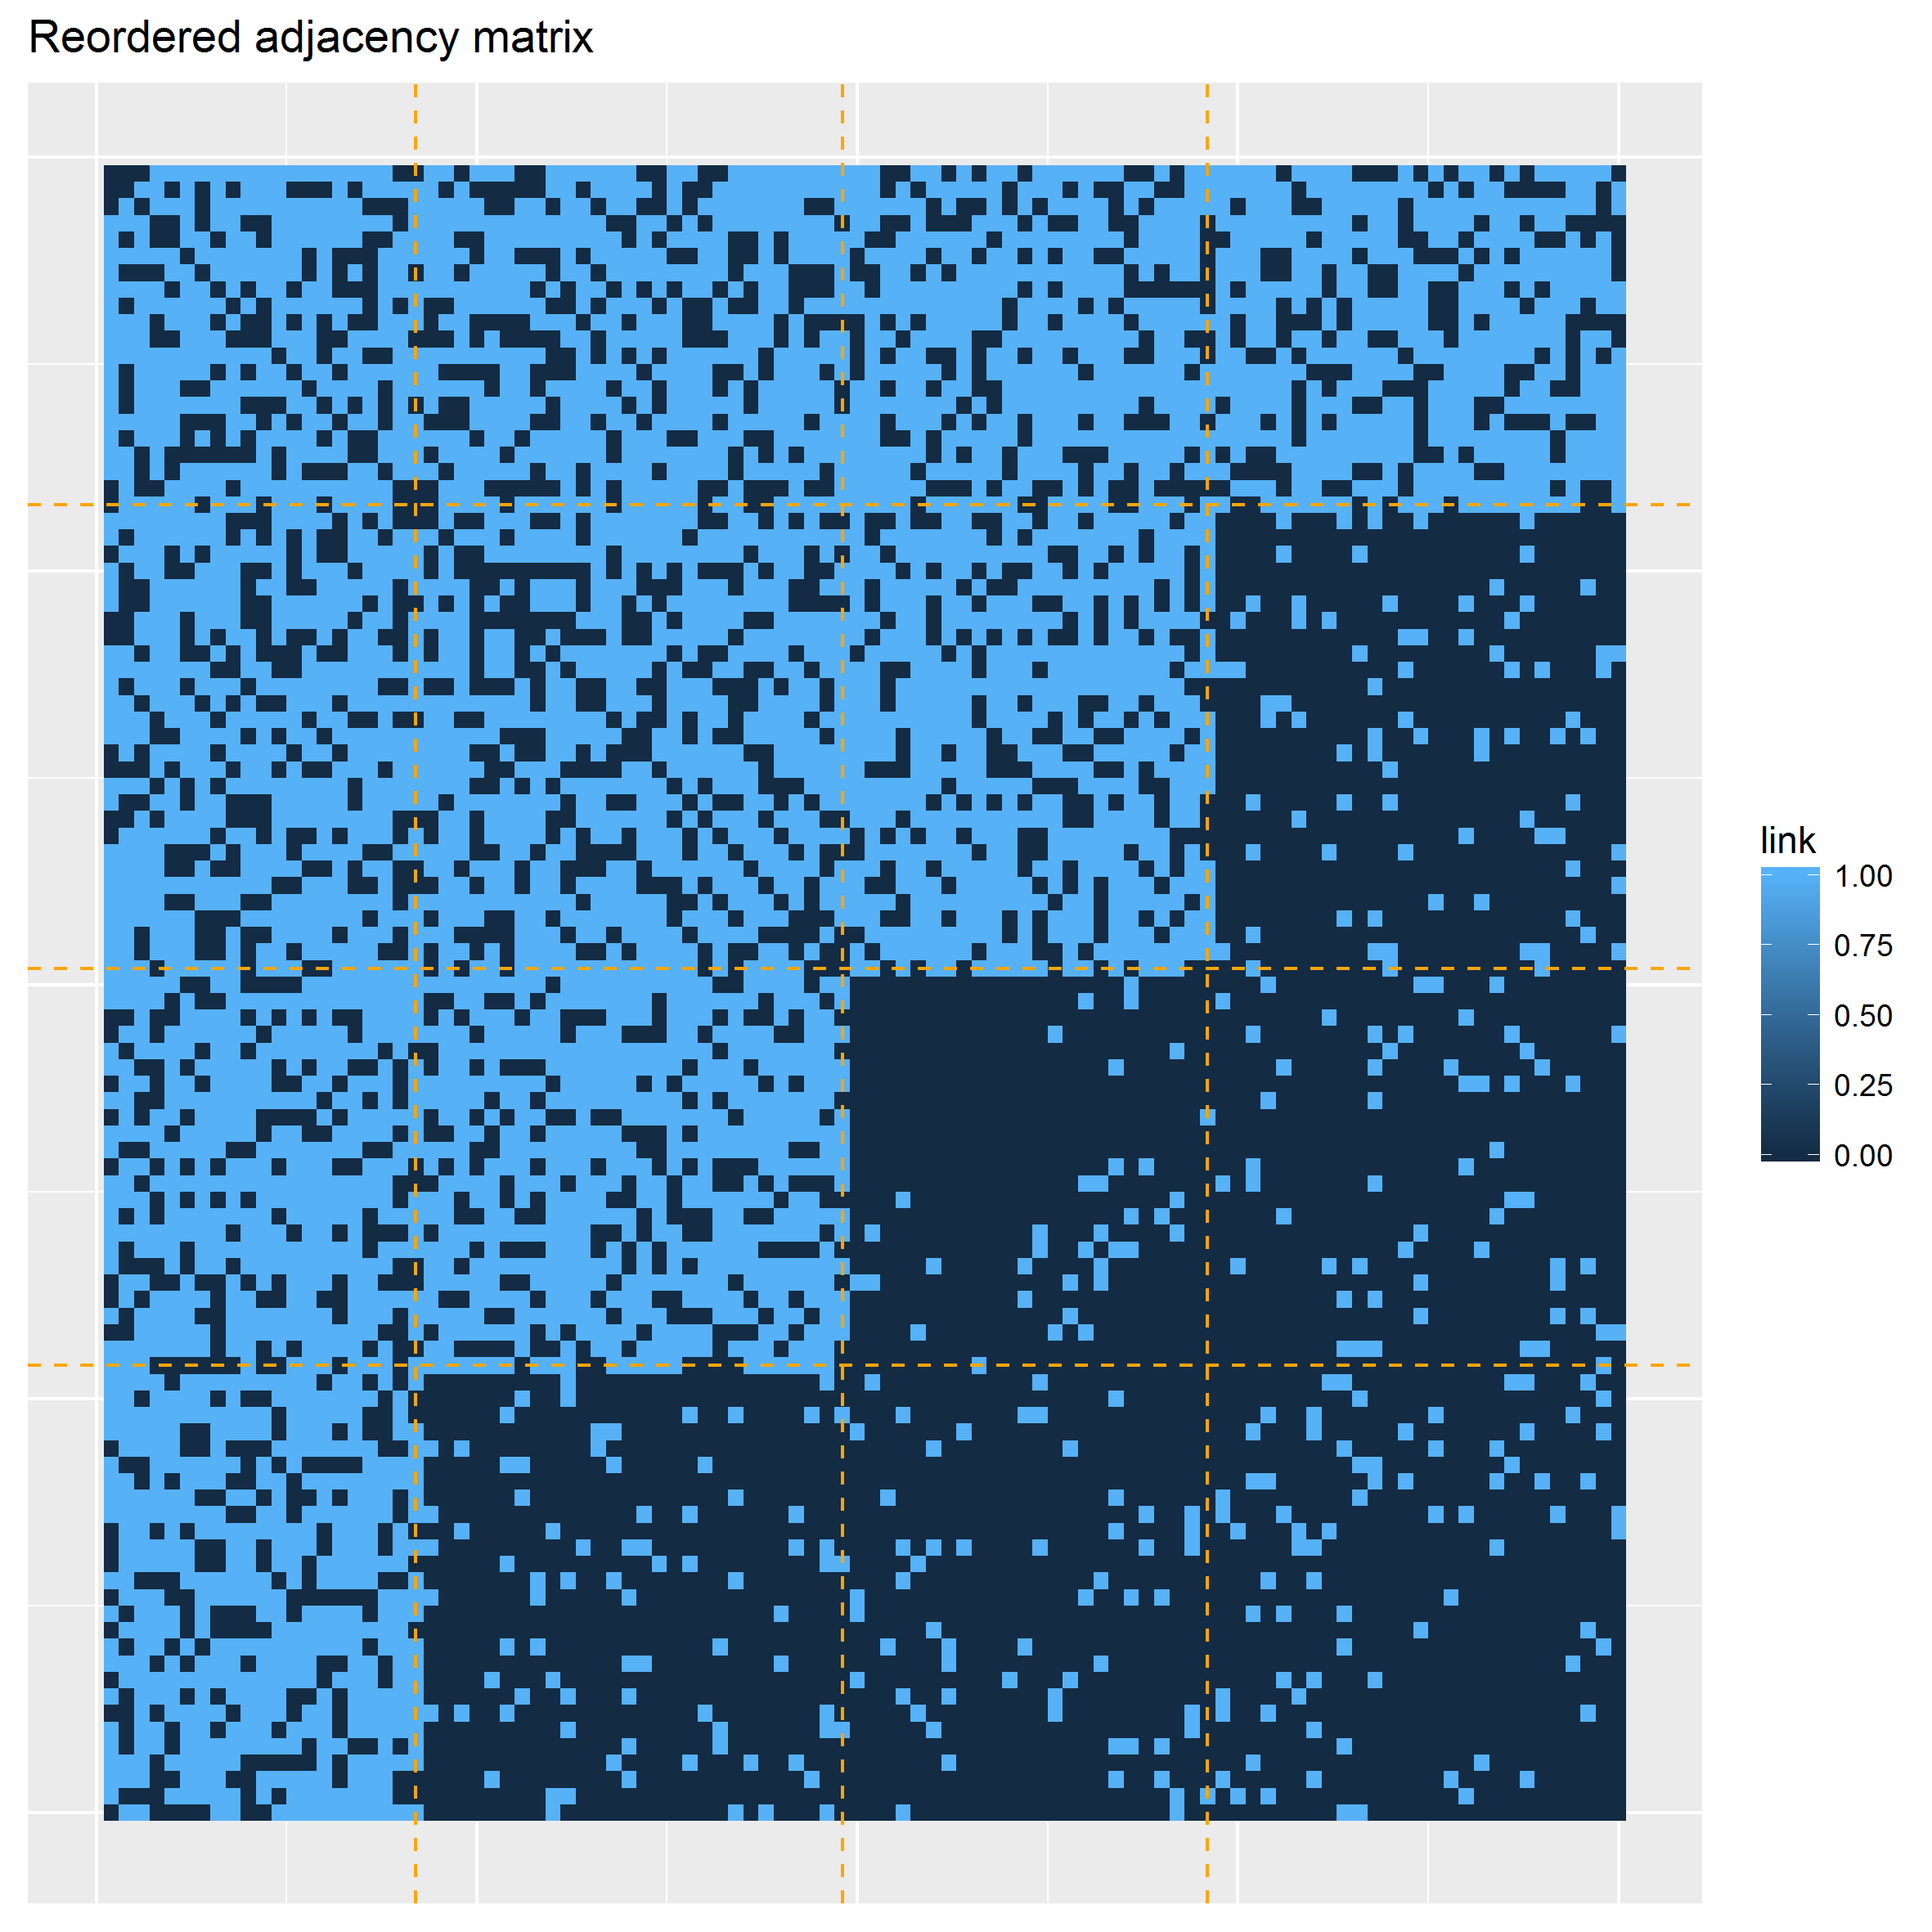
\includegraphics[scale=.2]{sbm/Nested_reordered_adja_with_groups.png}&
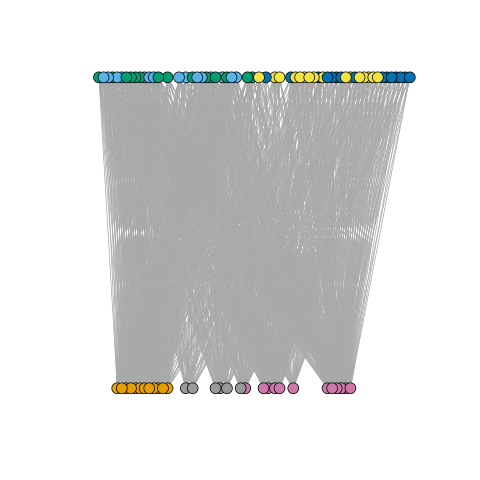
\includegraphics[scale=.2]{sbm/Nested_graphe_with_colors.png} 
 \end{tabular}

\end{frame}



%====================================================================
\begin{frame}  \frametitle{Statistical inference}
 %====================================================================
    \begin{center}
  \begin{overlayarea}{\textwidth}{.5\textheight}
      \begin{columns}
        \begin{column}{.45\paperwidth}
        \begin{tikzpicture}
          %% UN GRAPH

          \tikzstyle{every edge}=[-,>=stealth',shorten >=1pt,auto,thin,draw]
          \tikzstyle{every state}=[draw=none,text=white,scale=0.65, font=\scriptsize, transform shape]
          \tikzstyle{every node}=[fill=lightgray]
          % premier cluster
          \node[state] (A1) at (0,0.5) {N1};
          \node[state] (A2) at (1,0.5) {N2};
          \node[state] (A3) at (.5,1.5) {N3};

          \path (A2) edge [bend left] node[fill=white,below=.1cm]
          {}
          (A1)
          (A1) edge [bend left] (A3)
          (A3) edge [bend left] (A2);

          \tikzstyle{every node}=[fill=blue!80!black]
          \foreach \angle/\text in {234/N1, 162/N2, 90/N3, 18/N4, -54/N5} {
            \node[fill=lightgray,state,xshift=5cm,yshift=3.5cm]     (\text)    at
            (\angle:1cm) {\text};
          }
          \path (B2) edge (B5)
          (B1) edge (B4);
          \foreach \from/\to in {1/2,2/3,4/5,5/1}{
            \path (B\from) edge [bend left] (B\to);
          }

          \path    (B3)    edge     [bend    left]    node[fill=white]
          {}  (B4) ;
          
          \tikzstyle{every node}=[fill=lightgray]
          % troisime cluster
          \node[state] (C1) at (3,-.5) {N1};
          \node[state] (C2) at (4,0) {N2};

          \path (C1) edge [bend right] (C2);

          % inter cluster
          \path (A3) edge [bend right]  (B2)
          (A3)    edge    [bend    left]    node[fill=white]
          {}
          (B3)
          (C2) edge [bend right] node[fill=white,right]
          {}
          (B4)
          (A2) edge [bend right] node[fill=white]
          {}
          (C1);
        \end{tikzpicture}
        \end{column}
        \begin{column}{.5\paperwidth}
          \begin{small}
            \begin{block}{Stochastic Block Model}
              Let $n$ nodes divided into
              \begin{itemize}
              \item
                $\mathcal{K}=\{\textcolor{yellow!40!orange}{\bullet},\textcolor{blue!80!black}{\bullet},\textcolor{green!50!black}{\bullet}\}$,
                $\text{card}(\mathcal{K})$ known
              \item  $\pi_\bullet  =  ?$,
              \item      $\alpha_{\textcolor{yellow!40!orange}{\bullet}\textcolor{blue!80!black}{\bullet}}     =      ?$
              \end{itemize}
            \end{block}
          \end{small}
        \end{column}
      \end{columns}
    \end{overlayarea}
    \end{center}
    \medskip

    
   \cite{nowickiSnijders2001}, \cite{daudin2008mixture} 
    
    \bigskip
    
\textcolor{mygreen}{R package: blockmodels, sbm}
%     
%     \begin{thebibliography}{99}
%       \begin{scriptsize}
%       \bibitem[NS]{NS} Nowicki, Snijders, JASA, 2001 \newblock Estimation and prediction for
%         stochastic   blockstructures.
%         \textcolor{black}{} 
%       \bibitem[DRP]{DRP}   Daudin,  Picard,   Robin,  Statistics   and
%         Computing, 2008 \newblock A mixture model for random graphs. 
%       \end{scriptsize}
%   \end{thebibliography}

\end{frame}

%====================================================================
\begin{frame}\frametitle{Statistical inference} 
%====================================================================

From.... 

\centering
\begin{tabular}{cc}
 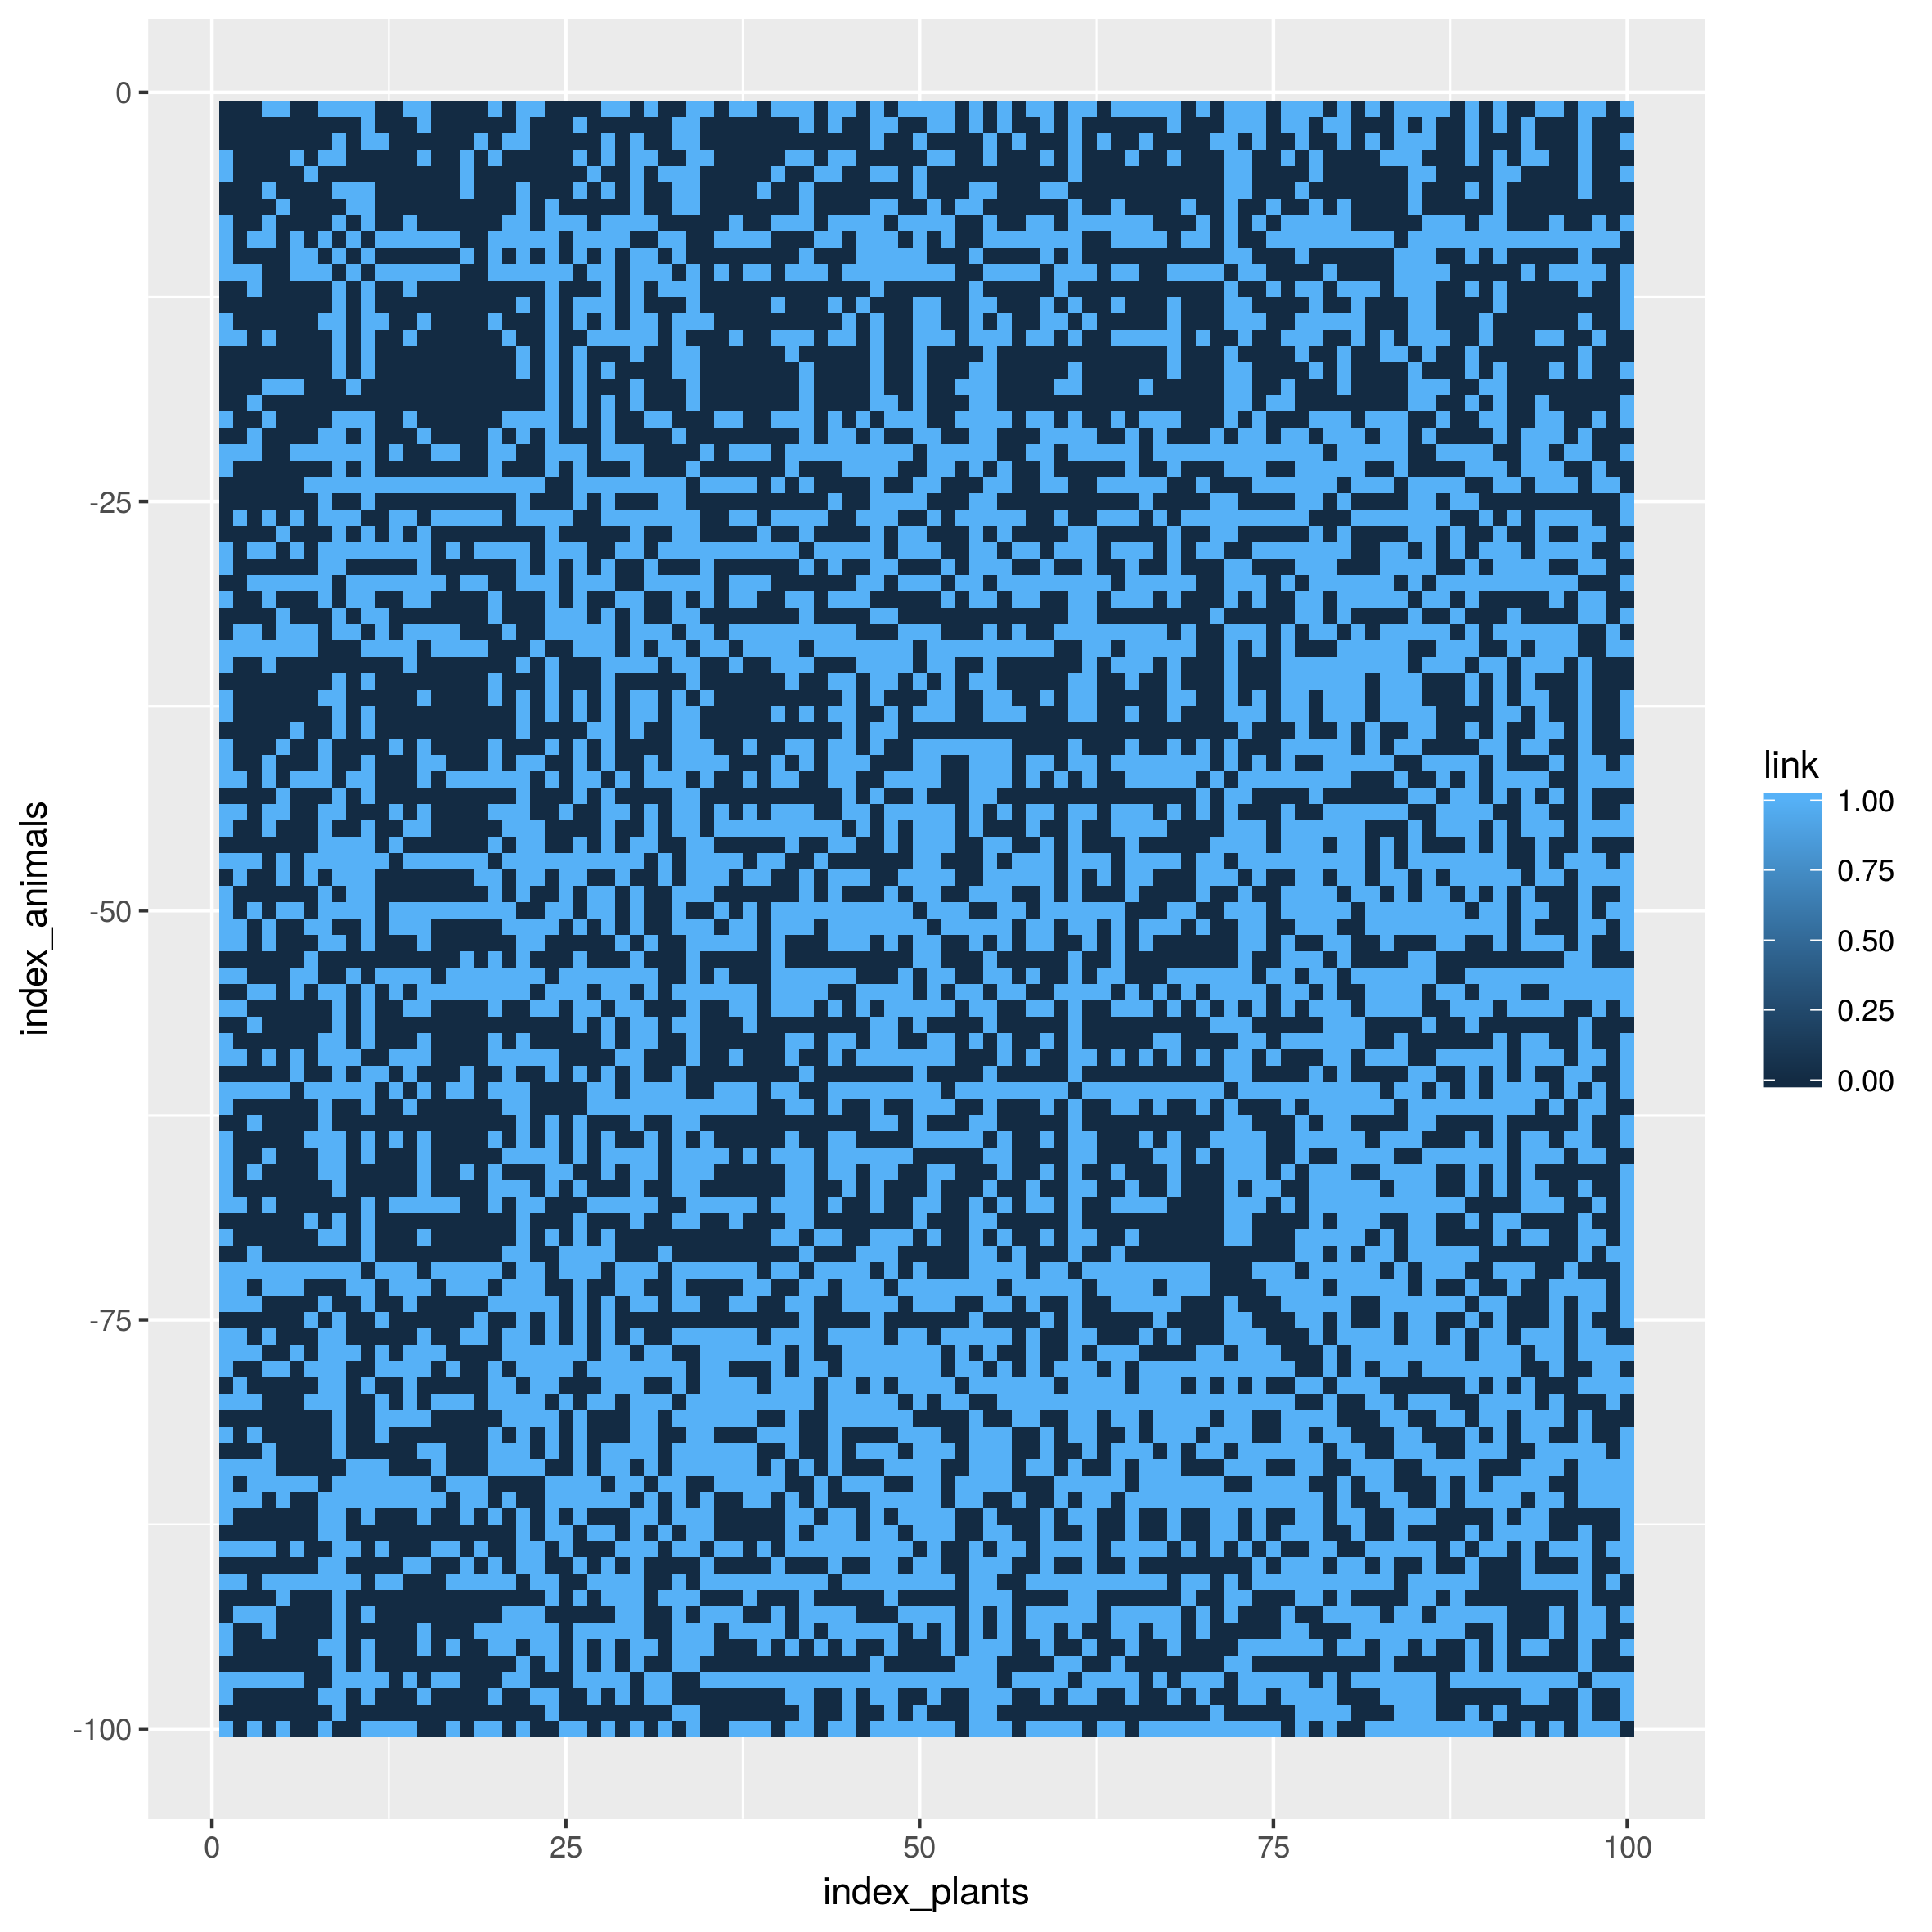
\includegraphics[scale=.2]{sbm/Nested_adja.png}&
 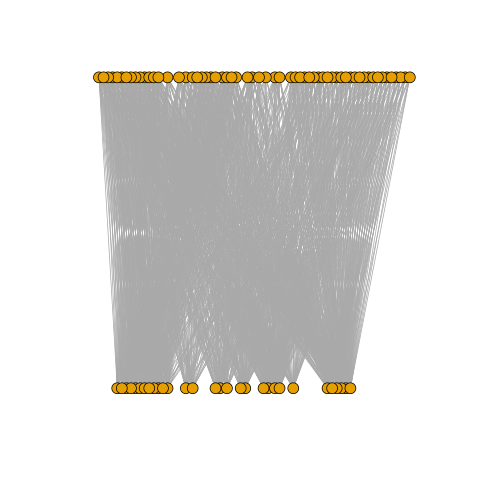
\includegraphics[scale=.2]{sbm/Nested_graphe_without_colors.png}
\end{tabular}
\end{frame}


%====================================================================
\begin{frame}\frametitle{Statistical inference} 
%====================================================================
... to 

\centering
\begin{tabular}{cc}
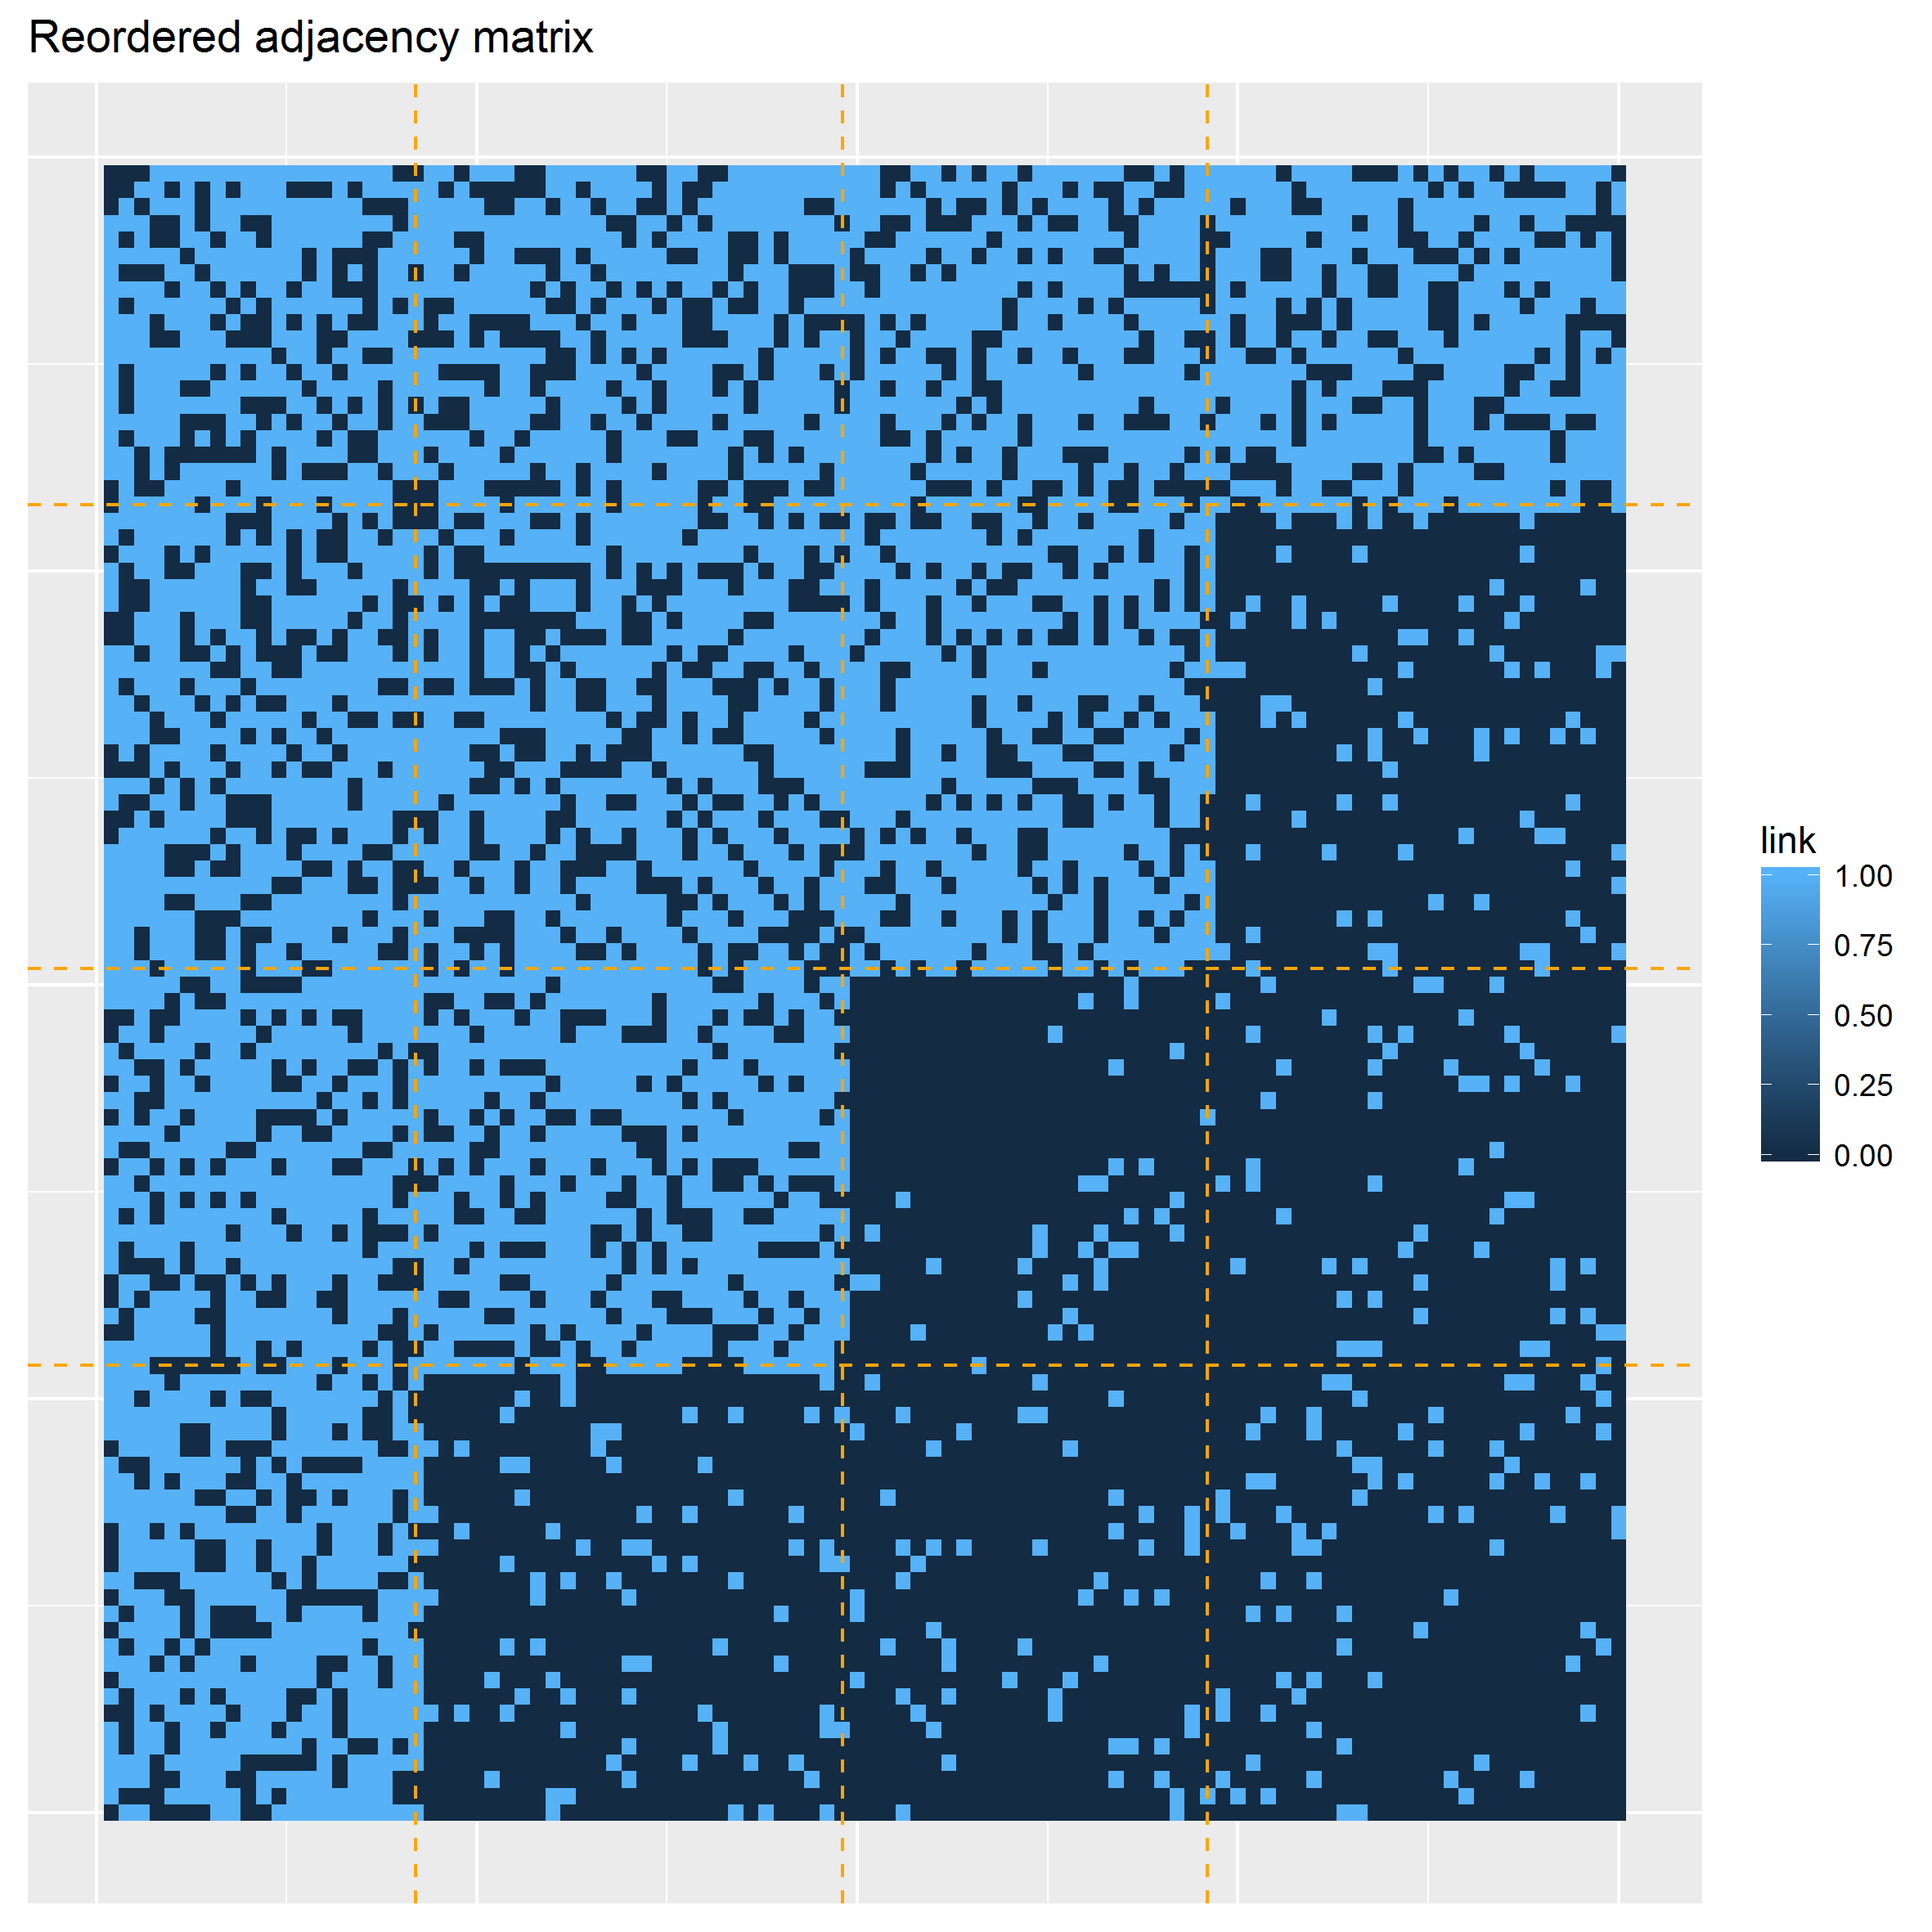
\includegraphics[scale=.2]{sbm/Nested_reordered_adja_with_groups.png}
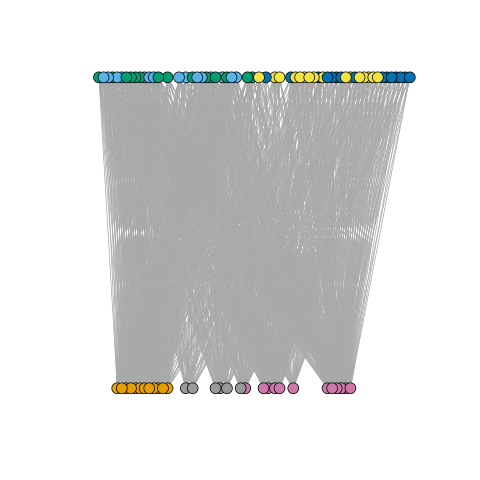
\includegraphics[scale=.2]{sbm/Nested_graphe_with_colors.png}
\end{tabular}

\begin{block}{Tasks}
\begin{itemize}
\item Find the clusters
\item Find the number of clusters
\item Practical implementation
\item Theoretical results
\end{itemize}
\end{block}

 

\end{frame}



%====================================================================
\subsection[LBM]{Latent block models}
%====================================================================

\begin{frame}{Probabilistic model for binary  bipartite networks}

Let $Y_{ij}$ be a bi-partite network. Individuals in row and cols are not the same. 

\begin{block}{Latent variables : bi-clustering}
\begin{itemize}
\item Nodes $i= 1,\dots,n_1$   partitionned into $K_1$ clusters,  nodes $j= 1,\dots,n_2$  partitionned into $K_2$ clusters
\item $$\begin{array}{cl}
Z^1_i = k & \mbox{if node $i$ belongs to cluster (block) $k$}\\
Z^2_j = \ell & \mbox{if node $j$ belongs to cluster (block) $\ell$}
\end{array}$$
\item $Z^1_i, Z^2_j$ independent variables
$$ \mathbb{P}(Z^1_i = k) = \pi^1_k,\quad  \mathbb{P}(Z^2_j = \ell) = \pi^2_\ell$$
\end{itemize}
\end{block}

\end{frame}

%====================================================================
\begin{frame}{Probabilistic model for binary  bipartite networks}
%====================================================================


\begin{block}{Conditionally to $(Z^1_i)_{i=1,\dots,n_1},(Z^2_j)_{j=1,\dots,n_2}$... }

$(Y_{ij})$ independent and 
\begin{eqnarray*}
 Y_{ij}  | Z^1_i, Z^2_j \sim  \mathcal{B}ern(\alpha_{Z^1_i,Z^2_j}) \quad \Leftrightarrow \quad   \mathbb{P}(Y_{ij} = 1 | Z^1_i = k, Z^2_j = \ell)  =  \alpha_{k\ell}
\end{eqnarray*}
\end{block}
 

\textcolor{mygreen}{\cite{Govaert2008}}

\end{frame}

%====================================================================
\begin{frame}\frametitle{Latent Block Model : illustration}
%====================================================================
 \begin{center}
    \begin{overlayarea}{\textwidth}{.5\textheight}
      \begin{columns}
        \begin{column}{.45\paperwidth}
        \centering
        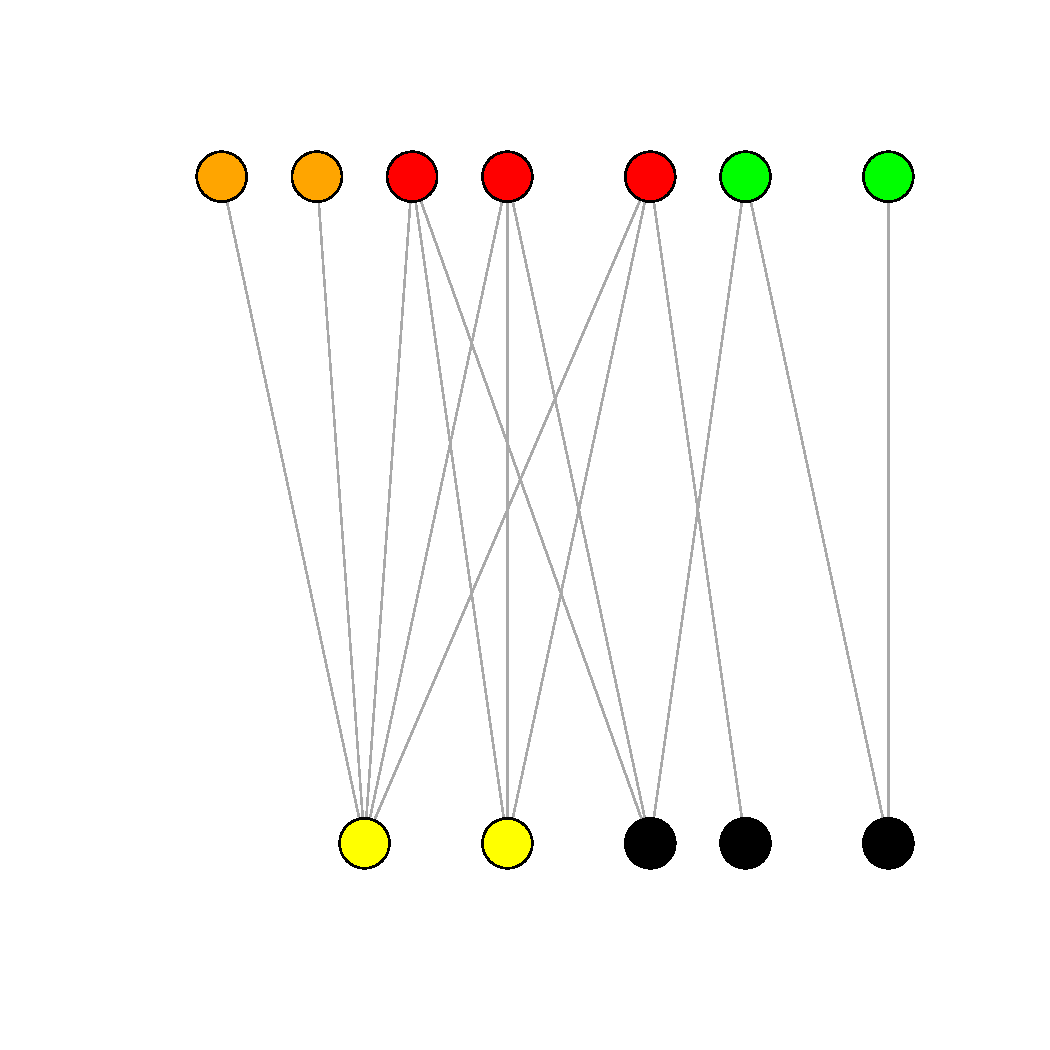
\includegraphics[scale=.3]{LBM_exemple.pdf}
        \end{column}
        \begin{column}{.5\paperwidth}
          \begin{small}
            \begin{block}{Latent Block Model}
              \begin{itemize}
              \item
                $n_1$ row nodes $\mathcal{K}_1=\{\textcolor{red}{\bullet},\textcolor{orange}{\bullet},\textcolor{green}{\bullet}\}$
                classes
              \item  $\pi^1_\bullet  =  \mathbb{P}(i  \in  \bullet)$,
                $\bullet\in\mathcal{K}_1,i=1,\dots,n$
              \item $n_2$ column nodes $\mathcal{K}_2=\{\textcolor{yellow}{\bullet},\textcolor{black}{\bullet}\}$
                classes
               \item  $\pi^2_\bullet  =  \mathbb{P}(j  \in  \bullet)$,
                $\bullet\in\mathcal{K}_2,j=1,\dots,m$
              \item      $\alpha_{\textcolor{red}{\bullet}\textcolor{yellow}{\bullet}}     =      \mathbb{P}(i
                \leftrightarrow j | i\in\textcolor{red}{\bullet},j\in\textcolor{yellow}{\bullet})$
              \end{itemize}
            \end{block}
          \end{small}
        \end{column}
      \end{columns}
    \end{overlayarea}
  \end{center}
  
%\begin{eqnarray*}
%&(Z_i) &  \ \sim^{\text{iid}} \mathcal{M}(1,\alpha) \ \text{et} \  Z_{i} \in \{1,...,Q\}, \\ 
% &(Y_{ij})&| \ \{Z_{i},Z_{j}\} \sim^{\text{ind}} \mathcal{B}(\pi_{Z_{i}Z_{j}}).\\
%\end{eqnarray*}

% Proposition Julien
\begin{align*}
Z^1_i = \mathbf{1}_{\{i \in \bullet\}}  \ & \sim^{\text{iid}} \mathcal{M}(1,\bpi^1), \quad \forall\bullet \in \mathcal{Q}_1, \\ 
Z^2_j=\mathbf{1}_{\{j \in \bullet\}}  \ & \sim^{\text{iid}} \mathcal{M}(1,\bpi^2), \quad \forall\bullet \in \mathcal{Q}_2, \\
Y_{ij} \ | \ \{i\in\textcolor{red}{\bullet},j\in\textcolor{yellow}{\bullet}\}
& \sim^{\text{ind}} \mathcal{B}ern(\alpha_{\textcolor{red}{\bullet}\textcolor{yellow}{\bullet}})\\
\end{align*}


\textcolor{mygreen}{\cite{Govaert2008}} and 
\textcolor{mygreen}{R package: blockmodels, sbm} as well.

\end{frame}


%====================================================================
\subsection{Some possible extensions}
%====================================================================


\begin{frame}\frametitle{Valued-edge networks}
%====================================================================

\begin{block}{Values-edges networks}
 Information on edges can be something different from presence/absence.
 It can be:
 \begin{enumerate}
  \item a count of the number of observed interactions,
  \item a quantity interpreted as the interaction strength,
  \end{enumerate}

 \end{block}

 \bigskip
 
 


\begin{block}{ Natural extensions of SBM and LBM}
 \begin{enumerate}
  \item Poisson distribution: $Y_{ij} \ | \ \{i\in\textcolor{yellow!40!orange}{\bullet},j\in\textcolor{blue!80!black}{\bullet}\}
\sim^{\text{ind}} \mathcal{P}(\lambda_{\textcolor{yellow!40!orange}{\bullet}\textcolor{blue!80!black}{\bullet}})$,
 \item Gaussian distribution: $Y_{ij} \ | \ \{i\in\textcolor{yellow!40!orange}{\bullet},j\in\textcolor{blue!80!black}{\bullet}\}
\sim^{\text{ind}} \mathcal{N}(\mu_{\textcolor{yellow!40!orange}{\bullet}\textcolor{blue!80!black}{\bullet}},\sigma^2)$,
\textcolor{mygreen}{\cite{mariadassou2010uncovering}}
\item More generally, 
  $$Y_{ij} \ | \ \{i\in\textcolor{yellow!40!orange}{\bullet},j\in\textcolor{blue!80!black}{\bullet}\}
\sim^{\text{ind}} \mathcal{F}(\theta_{\textcolor{yellow!40!orange}{\bullet}\textcolor{blue!80!black}{\bullet}})$$
 \end{enumerate}
 \end{block}
 \bigskip

\end{frame}

%====================================================================
\begin{frame} \frametitle{Multiplex networks}
%====================================================================
Several kind of interactions between nodes . 
For instance : 


\begin{itemize}
\item Love and friendship
\item Working relations and friendship
\item  In ecology : mutualistic and competition
\end{itemize}


\begin{block}{Block model for multiplex networks}

$Y_{ij} \in \{0,1\} ^ Q = (Y_{ij}^a, Y_{ij}^b)$, $\forall w \in \{0,1\}^2$ 



$$\mathbb{P}(Y^a_{ij},Y^b_{ij} = w  | Z_i  = k, Z_j = \ell)  = \alpha^w _{k\ell}$$

\end{block}

\textcolor{mygreen}{
\cite{kefi}, \cite{barbillon2017stochastic}}

In \textcolor{mygreen}{R package: blockmodels, sbm} when two relations are at stake.
 

 \textbf{Remark:} a particular case of multiplex network is dynamic network, \textcolor{mygreen}{\cite{matias2017statistical}}.
 

 \end{frame}
%==================================================================== 
\begin{frame} \frametitle{Taking into account covariates}
%==================================================================== 
 Sometimes covariates are available. They may be on:
 \begin{itemize}
  \item nodes,
  \item edges,
  \item both.
 \end{itemize}

 
 
 \begin{enumerate}
  \item They can be used a posteriori to explain blocks inferred by SBM.
  \item Extension of the SBM which takes into account covariates. Blocks are structure of interaction which is not 
  explained by covariates !

 \end{enumerate}


 If covariates are sampling conditions, case 2  be  may more interesting.
 
\end{frame}

%====================================================================
\begin{frame}\frametitle{SBM with covariates}
%====================================================================

\begin{itemize}
\item As before :  ($Y_{ij}$) be an adjacency matrix 
\item  Let   $x^{ij} \in \mathbb{R}^p$  denote covariates describing the pair $(i,j)$
\end{itemize}

\begin{block}{Latent variables : as before }
\begin{itemize}
\item The nodes $i= 1,\dots,n$ are partitioned into $K$ clusters
\item $Z_i$ independent variables
$$ \mathbb{P}(Z_i = k) = \pi_k$$
\end{itemize}
\end{block}
 
\begin{block}{Conditionally to $(Z_i)_{i=1,\dots,n}$... }

$(Y_{ij})$ independent and 
\begin{eqnarray*}
 Y_{ij}  | Z_i, Z_j&\sim&   \mathcal{B}ern(\mbox{logit}(\alpha_{Z_i,Z_j} + \beta \cdot x_{ij}) ) \quad \mbox {if binary data} \\
 Y_{ij}  | Z_i, Z_j  &\sim&  \mathcal{P}(\exp(\alpha_{Z_i,Z_j} + \beta  \cdot x_{ij}) ) \quad \mbox {if counting data} 
\end{eqnarray*}
\end{block}


If $K = 1$ : all the connection heterogeneity is explained by the covariates. 
 \end{frame}

%====================================================================
\section{Inference}
%====================================================================
\begin{frame}\frametitle{Statistical Inference}
%====================================================================
\begin{itemize}
\item Selection of the number of clusters $K$ for SBM  or $K_1,K_2$ for LBM
\item Estimation of the parameters $\mathbf{\pi}, \btheta$ for a given number of clusters
\item Clustering $\hat \bZ$
\end{itemize}

\end{frame}


%====================================================================
\subsection{Parameters estimation}
%====================================================================

\begin{frame} \frametitle{Likelihood for SBM}
For directed network .

 \begin{block}{Complete  likelihood $(\bY)$  et  $(\bZ)$}
 \begin{eqnarray}\label{eq:lik}
\ell_c(\bY,\bZ; \theta) &=& p(\bY | \bZ; \balpha) p(\bZ ; \bpi)\nonumber  \\
&=& \prod_{(i \neq j) = 1}^n f_{\alpha_{Z_i,Z_j}}(Y_{ij}) \times   \prod_{i=1}^n  \pi_{Z_i} \nonumber  \\
&=& \prod_{(i \neq j) = 1}^n\prod_{k=1}^K \prod_{\ell=1} ^K \left(f_{\alpha_{k,\ell}}(Y_{ij})\right)^{\ind_{Z_i=k} \ind_{Z_j=\ell}} \times   \prod_{i=1}^n \prod_{k=1}^K   (\pi_{k})^{\ind_{Z_i=k}} \nonumber  
%&=& \prod_{i \neq j = 1}^n \alpha_{Z_i,Z_j}^{Y_{ij}} (1-  \alpha_{Z_i,Z_j})^{1- Y_{ij}}    \prod_{i=1}^n \pi_{Z_i} \nonumber\\
\end{eqnarray}
 
 \end{block}
 

\begin{block}{Marginal likelihood $(\bY)$}
\begin{equation}\label{eq:vraismarg}
\log \ell(\bY; \theta) =\log \sum_{\bZ \in \boldsymbol{\mathcal{Z}}} \ell_c(\bY,\bZ; \theta) \,.
\end{equation}
 \end{block}
 

 \end{frame}
 

 
%====================================================================
\begin{frame}{Marginal likelihood  : remark }
%====================================================================
 
 $$
\log \ell(\bY; \theta) =\log \sum_{\bZ \in \boldsymbol{\mathcal{Z}}} \ell_c(\bX,\bZ; \theta) \,.
$$
 
  \begin{block}{Remark}
$\boldsymbol{\mathcal{Z}} =   \{1,\dots, K\}^{n}$ \color{dgreen} $\Rightarrow$ \color{black}  when  $K$ and $n$ increase, impossible to compute. 
 \end{block}
 
\color{dgreen} \textbf{Standard tool to maximize the likelihood when latent variables involved} \color{black} : EM  algorithm.  
 
 \end{frame}
 
%====================================================================
\begin{frame}{From EM to variational EM}
%====================================================================
 
\begin{block}{Standard EM}
At iteration $(t)$ : 
\begin{itemize}
 \item[$\bullet$]\textbf{Step E}: compute 
 $$ Q(\theta | \theta^{(t-1)}) =   \mathbb E_{\color{dgreen}\bZ | \bX, \theta^{(t-1)} } \left[\log \ell_c(\bY,\bZ; \theta)  \right] $$
 \item[$\bullet$]\textbf{Step M}: 
 $$ \theta^{(t)} = \arg \max_{\theta} Q(\theta | \theta^{(t-1)})$$
 \end{itemize}
% 
%
% 
\end{block}
 
 \end{frame}
%====================================================================
\begin{frame}{Limitations of standard EM}
%====================================================================

 \begin{center}
%   \includegraphics[scale=.3, clip=true, trim=0 335 65 0]{../Figures/HMModel}
  \begin{tikzpicture}
  \node[hidden] (Z1) at (0*\edgeunit, 2*\edgeunit) {$Z_1$};
  \node[hidden] (Z2) at (-2*\edgeunit,  0.5*\edgeunit) {$Z_2$};
 \node[hidden] (Z3) at (2*\edgeunit, 0*\edgeunit) {$Z_3$};

 
  \node[observed] (Y12) at (0*\edgeunit, 1*\edgeunit) {$Y_{12}$};
 \node[observed] (Y13) at (1*\edgeunit, 1*\edgeunit) {$Y_{13}$};
  \node[observed] (Y21) at (-1*\edgeunit, 0*\edgeunit) {$Y_{21}$};

  \node[observed] (Y23) at (1*\edgeunit, 0*\edgeunit) {$Y_{23}$};

  \node[observed] (Y31) at (-1*\edgeunit, -1*\edgeunit) {$Y_{31}$}; 
  \node[observed] (Y32) at (0*\edgeunit, -1*\edgeunit) {$Y_{32}$};


 
  \draw[arrow] (Z1) to (Y12);
  \draw[arrow] (Z1) to (Y21);
  \draw[arrow] (Z1) to (Y31);
  \draw[arrow] (Z1) to (Y13);
  
  \draw[arrow] (Z2) to (Y23);
  \draw[arrow] (Z2) to (Y32);
 
  \draw[arrow] (Z2) to (Y12);
  \draw[arrow] (Z2) to (Y21);
  
  
  \draw[arrow] (Z3) to (Y13);
  \draw[arrow] (Z3) to (Y23);
  \draw[arrow] (Z3) to (Y31);
  \draw[arrow] (Z3) to (Y32);
 
  
  \end{tikzpicture}
  \end{center}
  
\begin{itemize}
\item Step $E$ requires the computation of    $ \mathbb E_{\color{dgreen}\bZ | \bX, \theta^{(t-1)} } \left[\log \ell_c(\bX,\bZ; \theta)  \right] $
 \item However, once conditioned by par  $\bX$,  the  $\bZ$ are not independent anymore: complex  distribution if    $K$ and $n$ big. 
 

  
 
 \begin{eqnarray*}
  p(\bZ | \bY; \theta) & \propto& p(\bY | \bZ; \theta) p(\bZ | \theta)\\
  &\propto&  \prod_{i,j=1}^n f(Y_{ij};\alpha_{Z_i Z_j})\prod_{i}^n \pi_{Z_i}   
 \end{eqnarray*}
Impossible to separate to get $\prod_{i=1}\phi_i(Z_i)$
  \end{itemize}
 \end{frame}
 
%====================================================================
 \begin{frame}{Variational EM  : maximization of a lower bound}
%====================================================================

\textcolor{dgreen}{\textbf{Idea}} : replace the complicated distribution $p(\cdot | \Xall; \theta) = [\bZ | \bX, \theta]$ by a simpler one. 


Let $\mathcal{R}_{\Xall,\btau}$ be any distribution on   $\Zall$


\begin{block}{Central identity}
\begin{eqnarray*}
\mathcal{I}_{\theta}(\mathcal{R}_{\Xall,\btau}) &=& \log \ell(\Xall ; \theta) -   \mathbf{KL}[\mathcal{R}_{\Xall,\btau}, p(\cdot | \Xall; \theta)] \color{dgreen}\quad \leq   \log \ell(\Xall ; \theta)   \\
&=& \mathbb{E}_{\color{dgreen}\mathcal{R}_{\Xall,\btau}} \left[\log \ell_c(\bX,\bZ; \theta)   \right]  -   \sum_{\Zall} \mathcal{R}_{\Xall,\btau}(\bZ)  \log \mathcal{R}_{\Xall,\btau}({\bZ}) \\
&=& \mathbb{E}_{\color{dgreen}\mathcal{R}_{\Xall,\btau}} \left[\log \ell_c(\bX,\bZ; \theta)   \right]  +  \mathcal{H}\left(\mathcal{R}_{\Xall,\btau}(\bZ)\right) 
\end{eqnarray*}
\end{block} 

\textbf{Note that}:  
$$\mathcal{I}_{\theta}(\mathcal{R}_{\Xall,\btau})  = \log \ell(\Xall; \theta) \Leftrightarrow \mathcal{R}_{\Xall,\btau} = p(\cdot | \Xall; \theta)$$ 


\end{frame}
%====================================================================
 \begin{frame}[allowframebreaks]{Proof}
%==================================================================== 

By Bayes
\begin{eqnarray*}
\log \ell_c(\bX,\bZ; \theta)&=& \log  p(\bZ | \Xall; \theta) +   \log \ell(\Xall ; \theta)   \\
 \log \ell(\Xall ; \theta) &=& \log \ell_c(\bX,\bZ; \theta) -  \log  p(\bZ | \Xall; \theta)
\end{eqnarray*}

By integration against $\mathcal{R}_{\Xall,\btau}$ : 
\begin{eqnarray*}
 \mathbb{E}_{\color{dgreen}\mathcal{R}_{\Xall,\btau}} [ \log  \ell(\Xall ; \theta)] &=&  \mathbb{E}_{\color{dgreen}\mathcal{R}_{\Xall,\btau}} [\log \ell_c(\bX,\bZ; \theta)] -  \mathbb{E}_{\color{dgreen}\mathcal{R}_{\Xall,\btau}} [ \log  p(\bZ | \Xall; \theta)] \\
 \log \ell(\Xall ; \theta) &=&  \mathbb{E}_{\color{dgreen}\mathcal{R}_{\Xall,\btau}} [\log \ell_c(\bX,\bZ; \theta)] -  \mathbb{E}_{\color{dgreen}\mathcal{R}_{\Xall,\btau}} [ \log  p(\cdot | \Xall; \theta)]
\end{eqnarray*}

As a consequence: 
\begin{eqnarray*}
\mathcal{I}_{\theta}(\mathcal{R}_{\Xall,\btau}) &=& \log \ell(\Xall ; \theta) -   \mathbf{KL}[\mathcal{R}_{\Xall,\btau}, p(\cdot | \Xall; \theta)] \\
 &=& \mathbb{E}_{\color{dgreen}\mathcal{R}_{\Xall,\btau}} [\log \ell_c(\bX,\bZ; \theta)] -  \mathbb{E}_{\color{dgreen}\mathcal{R}_{\Xall,\btau}} [ \log  p(\bZ | \Xall; \theta)]  \\
&& -   \mathbb{E}_{\color{dgreen}\mathcal{R}_{\Xall,\btau}} \left[\log \frac{\mathcal{R}_{\Xall,\btau}(\bZ)} { p(\bZ | \Xall; \theta)}\right]\\
&=&  \mathbb{E}_{\color{dgreen}\mathcal{R}_{\Xall,\btau}} [\log \ell_c(\bX,\bZ; \theta)] -  \mathbb{E}_{\color{dgreen}\mathcal{R}_{\Xall,\btau}} [ \log  p(\bZ | \Xall; \theta)] \\
&& -   \underbrace{\mathbb{E}_{\color{dgreen}\mathcal{R}_{\Xall,\btau}} [\log \mathcal{R}_{\Xall,\btau}(\bZ)]}_{  \mathcal{H}\left(\mathcal{R}_{\Xall,\btau}(\bZ)\right) } +  \mathbb{E}_{\color{dgreen}\mathcal{R}_{\Xall,\btau}} [\log p(\bZ | \Xall; \theta)]
\end{eqnarray*}




  \end{frame}
%====================================================================
\begin{frame}{Variational EM }
%==================================================================== 

\begin{itemize}
\item Maximization of  $\log \ell(\Xall ; \theta)$  w.r.t.  $\theta$ replaced by maximization of the lower bound $\mathcal{I}_{\theta}(\mathcal{R}_{\Xall,\btau}) $  w.r.t.  $\tau$ and $\theta$. 
\item \textbf{Benefit} : we choose   $\mathcal{R}_{\Xall,\btau}$  such that the maximization calculus can be done explicitly
 \begin{itemize}
 \item In our case: mean field approximation : neglect dependencies between the  $(Z_i)$ 
 $$P_{\mathcal{R}_{\Xall,\btau}}(Z_i=k) = \tau_{ik}$$
  \end{itemize}


  % $\mathcal{R}_{\Xall,\btau}$ approximation of $p(\cdot | \Xall; \theta)$ in a certain class of distributions $\mathcal{P}$

 \end{itemize}
  \end{frame}
%====================================================================
\begin{frame}{Variational  EM}
%====================================================================

\begin{block}{Algorithm}
 \noindent At iteration $(t)$, given the current value  $(\theta^{(t-1)},\mathcal{R}_{\Xall, \btau^{(t-1)}})$,
\begin{enumerate}
\item[$\bullet$]\textbf{Step VE} Maximization w.r.t. $\tau$

\begin{eqnarray*}
\btau^{(t)}  &=&  \arg \max_{\btau  \in \mathcal{T}}  \mathcal{I}_{\theta^{(t-1)}}(\mathcal{R}_{\Xall,\btau})\\
 &=&  \arg \max_{\btau  \in \mathcal{T}}   \mathbb{E}_{\color{dgreen}\mathcal{R}_{\Xall,\btau}} \left[\log \ell_c(\bX,\bZ;  \theta^{(t-1)})   \right] +  \mathcal{H}\left(\mathcal{R}_{\Xall,\btau}(\bZ)\right) \\
&=&  \arg \max_{\btau  \in \mathcal{T}}  \log \ell(\Xall ; \theta^{(t-1)})  -  \mathbf{KL}[\mathcal{R}_{\Xall, \btau}, p(\cdot | \Xall; \theta^{(t-1)})]\\ 
&=& \arg \min_{\btau  \in \mathcal{T}}\mathbf{KL}[\mathcal{R}_{\Xall, \btau}, p(\cdot | \Xall; \theta^{(t-1)})]\\ 
 \end{eqnarray*}
 \end{enumerate}

 \end{block} 
 \end{frame}

 %====================================================================
 \begin{frame}{Variational  EM}
%====================================================================

\begin{block}{Algorithm}
\begin{enumerate}
 \item[$\bullet$]\textbf{Step M} Maximization  w.r.t.  $\theta$
 \begin{eqnarray*}
 \theta^{(t)} &=& \arg \max_{\theta}   \mathcal{I}_{\theta}(\mathcal{R}_{\Xall,\btau^{(t)}}) \\
 &=&   \arg \max_{\theta} \mathbb{E}_{\color{dgreen}\mathcal{R}_{\Xall,\btau^{(t)}}} \left[\log \ell_c(\bX,\bZ;  \theta)   \right]  +   \mathcal{H}\left(\mathcal{R}_{\Xall,\btau^{(t)}}(\bZ)\right)\\
&=&  \arg \max_{\theta} \mathbb{E}_{\color{dgreen}\mathcal{R}_{\Xall,\btau^{(t)}}} \left[\log \ell_c(\bX,\bZ;  \theta)   \right]  
 \end{eqnarray*}
 
\end{enumerate}

 \end{block} 
 \end{frame}
 
%====================================================================
 \begin{frame}[allowframebreaks]{VE-step for SBM}
%====================================================================
 
\begin{equation}
 \nonumber
\btau^{(t)} = \arg \min_{\btau}  \mathbf{KL}[\mathcal{R}_{\Xall,\tau}, p(\cdot | \Xall; \theta^{(t-1)})] = \arg \max_{\btau} \mathcal{I}_{\theta^{(t-1)}}(\mathcal{R}_{\Xall,\btau}) \,.
 \end{equation}
(we drop out the index $^{(t-1)}$ on $\theta$)

\begin{eqnarray*}
 \mathcal{I}_{\theta}(\mathcal{R}_{\Xall,\btau}) &=&   \sum_{\bZ} \mathcal{R}_{\Xall,\btau}(\bZ) \log \ell_c(\Xall, \bZ; \theta) -  \sum_{\Zall} \mathcal{R}_{\Xall,\btau}(\bZ)  \log \mathcal{R}_{\Xall,\btau}({\bZ})\,,
 \end{eqnarray*}
 with
 \begin{eqnarray*}
 \log \ell_c(\Xall, \bZ; \theta) &=& \log p(\Xall |  \bZ; \theta)+ \log  p(\bZ; \theta)\,,\\
 %&=&   \log \prod_{i,j,i\neq j}p(Y_{ij}|  Z_i,Z_j; \theta) + \log \prod_{i=1}^n \alpha_{Z_i}\,,\\
 &=& \sum_{i,j=1, i\neq j}^n  \log p(Y_{ij} |  Z_i,Z_j; \theta)  + \sum_{i=1}^n \log\pi_{Z_i}\,.\\
 &=& \sum_{i,j=1, i\neq j}^n \sum_{k,\ell=1}^K Z_{ik}Z_{j\ell}\log p(Y_{ij} |\alpha_{k\ell})+ \sum_{i=1}^n\sum_{k=1}^K Z_{ik} \log\pi_{k}
 \end{eqnarray*}
 
 
Integration of the $\bZ$ where $\bZ \sim \mathcal{R}_{\Xall,\btau}$% which means that $ \bZ= (Z_i)_{i=1\dots n} $ are independent variables such that $\P(Z_{i}=q) = \tau_{iq}$. We obtain:
 \begin{eqnarray*}
 \mathcal{I}_{\theta}(\mathcal{R}_{\Xall,\btau}) &=& \sum_{i,j=1, i\neq j}^n \sum_{k,\ell=1}^K \tau_{iq}\tau_{j\ell}\log p(Y_{ij} |\alpha_{k\ell})+ \sum_{i=1}^n\sum_{k=1}^K  \tau_{ik} \log\pi_{k} 
 \end{eqnarray*}

 
Maximization under the constraint: $\forall i =1 \dots n$, $\sum_{k=1}^K \tau_{ik}=1$.
 
 
 
\begin{itemize}
 
\item Derivatives of  $$\; \mathcal{I}_{\theta}(\mathcal{R}_{\Xall,\btau})  + \sum_{i=1}^n \lambda_i \left[ \sum_{k=1}^K \tau_{ik}-1\right]$$
 with respect to $(\lambda_i)_{i=1\dots n}$ and $(\tau_{ik})_{i=1\dots n, k=1 \dots K}$ where $\lambda_i$ are the Lagrange multipliers, 
 
 
 
\item Leads  to collection of equations:  for $i=1\dots n$ and $k=1\dots K$,

 \begin{equation}
  \nonumber
 \sum_{\ell=1}^K \sum_{j=1, j\neq i}^n  \log p(Y_{ij} | \alpha_{k\ell})\tau_{j\ell}   +   \log\pi_{k}  -   \log \tau_{ik} +1 + \lambda_i=0\,,
 \end{equation}
 
 \item Leads to the following fixed point problem:

 \begin{equation}
  \nonumber
  \widehat{\tau}_{ik} = e^{1+ \lambda_i} \alpha_k \prod_{j=1, j\neq i}^n \prod_{\ell=1}^K p(Y_{ij} | \alpha_{k\ell}) ^{\widehat{\tau}_{j\ell}}, \quad \forall  i =1 \dots n,  \forall  k=1 \dots K\,,
 \end{equation}
 which has to be solved under the constraints $\forall i =1 \dots n$, $\sum_{k=1}^K \tau_{ik}=1$. This optimization  problem is solved using a  standard fixed point algorithm.

 \end{itemize}
 
 \end{frame}
 
 %====================================================================
 \begin{frame}[allowframebreaks]{M-step for SBM}
%====================================================================

$$\theta^{(t)} = \arg \max_{\theta}   \mathcal{I}_{\theta^{(t)}}(\mathcal{R}_{\Xall, \btau^{(t)}}) $$

under the constraints: $ \sum_{k=1}^k \pi_k=1.$


Maximization with respect to $\bpi$ is quite direct:
$$
\widehat{\pi}_q = \frac{1}{n} \sum_{i=1}^n \widehat{\tau}_{ik}
$$ 
 
For the Bernoulli SBM: 

$$
\widehat{\alpha}_{k\ell} = \frac{\sum_{i,j=1,i\neq j}^n \widehat{\tau}_{ik}  \widehat{\tau}_{j\ell} Y_{ij}}{\sum_{i,j=1,i\neq j}^n  \widehat{\tau}_{ik}  \widehat{\tau}_{j\ell} }
$$

If the edge probabilities depend on covariates:
\begin{equation}
 \nonumber
 \mbox{logit}(p_{k\ell}) = \alpha_{k\ell} +  \beta \cdot x_{ij}\,,
\end{equation}
then the optimization of $ (\alpha_{k\ell})$ and $ (\beta)$ at step M of the VEM is not explicit anymore and one should resort  to optimization algorithms such as Newton-Raphson
algorithm.  
 
 \end{frame}
%====================================================================
\begin{frame}{In practice}
%====================================================================
\begin{itemize}
\item Really fast
\item Strongly depend on the initial values
\end{itemize}

\end{frame}
%==================================================================== 
 \subsection{Model selection}
%====================================================================
\begin{frame}{ Penalized likelihood criterion}
%====================================================================

 \begin{itemize}
 \item  Selection of the number of clusters  $K$ (or $K_1$, $K_2$ in the LBM)
\item   Integrated Classification Likelihood (ICL)   \textcolor{mygreen}{\cite{biernacki2000assessing}}
 

\begin{equation}\label{eq:ICL}
ICL(\M) =\log  \ell_c(\Xall,\hat{\bZ}; \hat \theta_{\bK})-  \pen(\M)
\end{equation}
 where  \begin{equation}\label{eq:Zhat}
\hat{Z}_i = \argmax_{k \in \{1, \dots, K\}}  \hat{\tau}_{ik}. 
\end{equation} 
\item   Integrated Complete Likelihood (ICL)  % \textcolor{mygreen}{\cite{biernacki2000assessing}}

 

\begin{equation}\label{eq:ICL}
ICL(\M) =\mathbb{E}_{p(\cdot | \bY, \hat \theta_{\bK})}[\log  \ell_c(\Xall,\hat{\bZ}; \hat \theta_{\bK})-  \pen(\M)
\end{equation}
 \end{itemize}

\end{frame}


%====================================================================
\begin{frame}{Expression of the penalization}
%====================================================================

\textcolor{dgreen}{ \textbf{For SBM } }

$$ pen_{\mathcal{M}} = \left\{ 
\begin{array}{ll}
- \frac{1}{2}\left\{ (K-1)\log(n)  +K^2   \log \left( n^2-n \right)\right\} & \mbox{for directed network}\\
 - \frac{1}{2}\left\{ \underbrace{(K-1)\log(n) }_{\mbox{\textcolor{dgreen}{Clust. }}} + \frac{K(K+1)}{2}   \log \left(\frac{ n^2-n }{2}\right)\right\} & \mbox{for undirected network}\\
\end{array}
\right.
$$
 

\textcolor{dgreen}{ \textbf{For LBM } }
%
\begin{eqnarray*}
 pen_{\mathcal{M}} =  -  \frac{1}{2}&& \left\{  \underbrace{ (K_1-1)\log(n_1) +  (K_2-1)\log(n_2)  }_{\mbox{\textcolor{dgreen}{Bi-Clust. }}} \right. \\
& &  + \left. \underbrace{ (K_1  K_2)    \log ( n_1   n_2)} _{\mbox{\textcolor{dgreen}{Connection }}} \right\} 
 \end{eqnarray*}

\end{frame}
 

%====================================================================
\begin{frame}{Advantages of ICL}
%====================================================================


 
\begin{itemize}
\item its capacity to outline the clustering structure in networks% in \cite{Daudinetal2008} (for simple networks),  \cite{keribin2015} (for bipartite networks)  or \cite{mariadassou2010} for valued networks.  
\item Involves a trade-off between goodness of fit and model complexity
\item ICL values :   goodness of fit  AND clustering  sharpness.
 
\end{itemize}

\end{frame}

 


  %------------------------------------------------------------------------------------------------------

 \begin{frame}{Comments on the   ICL versus BIC}

\begin{block}{Conjecture}
\begin{eqnarray*}
 BIC(\Mcal)  &=&  \log \ell(\Xall; \hat{\theta}, \Mcal) - \mbox{pen}(\Mcal)
\end{eqnarray*}
with the same penalty
 \end{block}

\begin{itemize}
\item Under this conjecture
\begin{eqnarray*}
 ICL(\Mcal)  &= & BIC(\Mcal)  +   \sum_{\Zall} p(\bZ | \Xall;\hat \theta_{\bK}) \log p(\bZ | \Xall; \hat \theta_{\bK})\\
 &=& BIC(\Mcal)  -   \mathcal{H}( p(\cdot | \Xall; \theta)) 
\end{eqnarray*}
\item As a consequence, because of the entropy,  ICL  will encourage clustering with well-separated groups 
\item 
$$ 
 \widehat{ICL}(\mathcal{M})  =BIC(\mathcal{M})  +   \sum_{\Zall} \mathcal{R}_{\Xall}(\bZ,\widehat{\btau})  \log \mathcal{R}_{\Xall,\widehat{\btau}}({\bZ}) -  \mathbf{KL}[\mathcal{R}_{\Xall,\widehat{\btau}}, p(\cdot | \Xall;\widehat{\theta})]\,. 
$$

\end{itemize}

 
 \end{frame}
 
 

   %------------------------------------------------------------------------------------------------------



\begin{frame}{Algorithm in practice}  
\begin{itemize}
\item Going trough the models and initiate VEM at the same time
\item Bounds on $K$ :  $\{K_{ \min},\dots, K_{\max}\}$
\end{itemize}

\begin{block}{Stepwise procedure}
Starting from  $K$

\begin{itemize}
\item \textbf{Split} : if $K<K_{\max}$
\begin{itemize}
\item Maximize the likelihood (lower bound) of  $\mathcal{M}_{K+1}$
\item  $K$ initializations of the VEM are proposed :  split each cluster into $2$ clusters  
\end{itemize}
\item \textbf{Merge} :  If $K>K_{\min}$
\begin{itemize}
\item Maximize the likelihood (lower bound) of   model  $\mathcal{M}_{K-1}$
\item  $\frac{K(K-1)}{2}$ initializations of the VEM are proposed :   merging all the possible pairs of  clusters 
 \end{itemize}
\end{itemize}

\end{block}
 \end{frame}


\begin{frame}\frametitle{Theoretical properties for SBM}
\begin{itemize}
\item Identifiability and a first consistency result by \color{blue} \cite{celisse2012consistency} \color{black}
\item Consistency of the posterior distribution of the latent variables \color{blue} \cite{mariadassou2015convergence} \color{black}
\item Consistency and properties of the variational estimators \color{blue} \cite{bickel2013asymptotic} \color{black}
\end{itemize}
\end{frame}
%--------------------------------------------------- 
\begin{frame}{Other extensions}

\begin{itemize}
\item  Time evolving networks \textcolor{mygreen}{Matias} 
\item  Multipartite, Multiplexe networks (\textcolor{mygreen}{R-package  sbm, Bar-Hen, Barbillon, Donnet}) 
\item Multilevel networks (individuals and organizations)  (\textcolor{mygreen}{Chabbert-Liddell})
 \item Missing data in the network,
\end{itemize}
\end{frame}

%------------------------------------------ 
\begin{frame}
 \frametitle{Probabilistic model for networks in a nutshell}
 
 SBM/LBM
 \begin{itemize}
  \item generative models,
  \item flexible,
  \item comprehensive models which can be linked to a lot of classical descriptors.
  
 \end{itemize}
\end{frame}

%------------------------------------------ 

\begin{frame}[allowframebreaks]{References}
\bibliographystyle{apalike}
 \small{\bibliography{biblioSlidesSBM}}
  \end{frame}
  
  
  




\end{document}


 
 
